\documentclass[12pt, a4paper, titlepage]{article}

\usepackage[utf8]{inputenc}     % Permite el uso de caracteres como ñ y acentos
\usepackage[spanish]{babel}     % Configura el documento en español
\usepackage{graphicx}           % Para manipular gráficos e imágenes en el documento
\usepackage{float}              % Permite forzar una ubicación exacta de imágenes con [H]
\usepackage{listings}           % Permite formato de fragmentos de código de programación
\usepackage[autostyle=false, style=english]{csquotes} % Permite escribir "" con \enquote{}
\usepackage[explicit]{titlesec} % Permite personalizar el estilo de los títulos y secciones
\usepackage{xcolor}             % Para definir y usar colores personalizados en texto
\usepackage{geometry}           % Para configuración de los márgenes y el tamaño de la página
\usepackage{lipsum}             % Para generar texto de relleno ("Lorem ipsum")
\usepackage{tocloft}            % Para personalizar el formato del índice
\usepackage{subfiles}           % Para incluir de otros archivos .tex en el main mediante \include{}
\usepackage[colorlinks=true, allcolors=blue, linktoc=all]{hyperref} % Crea enlaces dentro del documento 
\usepackage{bookmark}           % Mejora la administración de los marcadores (bookmarks) en documentos PDF generados
\usepackage{xr}                 % Permite referenciar elementos de otros documentos .tex



% Configuración de márgenes
\geometry{
    left=2.5cm,  % Margen izquierdo
    right=2.5cm, % Margen derecho
    top=3cm,     % Margen superior
    bottom=3cm   % Margen inferior
}


% Definimos una nueva forma de referirnos a las \section, \subsection y \subsubsection.
% Ahora en los subarchivos tex al llamarlas de esta forma aseguramos que en la
% Table of Contents (ToC) aparezcan los números de las secciones que seleccionemos
%     \subsection*{} hace que salga el titulo en formato subsection pero no aparece en el ToC
%     \numberedsubsection hará que si salga en la ToC
\newcommand{\numberedsection}[1]{%
  \stepcounter{section}%
  \section*{#1}%
  \addcontentsline{toc}{section}{\protect\numberline{\thesection}#1}%
}
\newcommand{\numberedsubsection}[1]{%
  \stepcounter{subsection}%
  \subsection*{#1}%
  \addcontentsline{toc}{subsection}{\protect\numberline{\thesubsection}#1}%
}
\newcommand{\numberedsubsubsection}[1]{%
  \stepcounter{subsubsection}%
  \subsubsection*{#1}%
  \addcontentsline{toc}{subsubsection}{\protect\numberline{\thesubsubsection}#1}%
}

\begin{document}

% PORTADA
\begin{titlepage}
    \centering
    {\bfseries\LARGE Universidad de Málaga\par}
    \vspace{1cm}
    {\scshape\Large ETSI Informática\par}
    \vspace{2cm}
    {\scshape\Huge Memoria de la\par}
    \vspace{0.1cm}
    {\scshape\Huge $1^{ra}$ iteración}
    \vspace{2cm}
    \begin{figure}[H]
        \centering
         
\includegraphics[width=0.30\linewidth]{assets/umaLogo.png}
    \end{figure}
    \vfill
    {\scshape\Large Ingeniería de Requisitos (2024$-$25)\par}
    \vfill
    {\Large Diego Sicre Cortizo\par}
    {\Large Pablo Ortega Serapio\par}
    {\Large Angel Nicolás Escaño López\par}
    {\Large Francisco Javier Jordá Garay\par}
    {\Large Janine Bernadeth Olegario Laguit\par}
    \vspace{1cm}
    {\Large Grupo 01}
    \vfill
    {\Large Noviembre 2024}
\end{titlepage}
% FIN PORTADA

% ÍNDICE
\tableofcontents % Crea el Índice
\thispagestyle{empty} % Quita el número de la primera página
\newpage
\listoffigures % Crea un Índice de figuras (registra imágenes)
\thispagestyle{empty}
\newpage
% FIN ÍNDICE


% CUERPO DEL DOCUMENTO
\setcounter{page}{4} % Inicia a contar las páginas a partir de {}

\phantomsection\numberedsection{RF2.1 Crear Producto}

\subsection*{Descripción}
Los usuarios deben de poder crear productos mientras sea posible, definiendo sus atributos y asignándoles sus respectivas categorías y relaciones.\par
\vspace{0.15cm}

\textbf{Pre-condición}\par
El usuario debe haber iniciado sesión en su cuenta en Mini PIM.\par
\vspace{0.15cm}

\textbf{Post-condición}
\begin{itemize}
    \item Caso de éxito: Todos los productos que el usuario creó se reflejan en la base de datos del sistema y en su interfaz gráfica.
    \item Caso mínimo: El sistema notifica al usuario el resultado de la acción de crear producto; exitosa o fallida.
\end{itemize}

\textbf{Prioridad: }
Alta
\vspace{0.15cm}

\textbf{Autor: }
Francisco Javier Jordá Garay\par
\vspace{0.15cm}

\textbf{Control de cambios: } Versión 1: Definición del caso de uso

\numberedsubsection{Escenario principal}
\begin{enumerate}
    \item El usuario se encuentra en el apartado de productos y selecciona la opción de \enquote{Añadir}.
    \item El sistema muestra el menú de creación solicitando al usuario:
    \begin{itemize}
        \item GTIN (atributo sistema $-$ comprueba validez de longitud)
        \item SKU (atributo sistema)
        \item Thumbnail (atributo sistema $-$ comprueba tamaño 200$\times$200px y formato)
        \item Label (atributo sistema $-$ comprueba máximo de 250 caracteres)
        \item Atributos (opcional $-$ comprueba máximo 5 nuevos atributos usuario)
        \item Categorías (opcional)
    \end{itemize}
    \item El usuario introduce los datos obligatorios y los que decida de opcionales y selecciona \enquote{Confirmar}.
    \item El sistema comprueba la validez de los datos introducidos por el usuario.
    \item El sistema almacena el producto creado en la base de datos registrando la fecha de creación.
    \item El sistema actualiza la información del total de datos registrados en la base de datos.
    \item El sistema muestra el apartado de \enquote{Productos} todos los recursos almacenados para esta sección.
\end{enumerate}

\numberedsubsection{Escenarios alternativos}
\begin{description}
    \item[2.a.] El sistema no puede almacenar el producto por superar el máximo de almacenamiento ligado al plan de suscripción del usuario.
    \begin{enumerate}
        \item[2.a.1] El sistema notifica al usuario que ha llegado al máximo de capacidad permitida en el plan de almacenamiento.
    \end{enumerate}

    \item[*.a] El usuario cancela la acción de crear un nuevo producto seleccionando la opción que cierra el menú de creación.
    \begin{enumerate}
        \item[*.a.1] El sistema regresa al apartado de \enquote{Productos}.
    \end{enumerate}

    \item[4.a] El sistema detecta un fallo en la comprobación de los datos obligatorios.
    \begin{enumerate}
        \item[4.a.1] El sistema notifica del error de comprobación al usuario mostrando el atributo del producto afectado.
        \item[4.a.2] El sistema regresa al menú de creación permitiendo edición de los datos.
    \end{enumerate}
\end{description}

\numberedsubsection{Casos de Prueba}
\underline{Escenario: Principal}\par
\vspace{0.15cm}
\textbf{Dado} que inicié sesión con mi cuenta de usuario correspondiente\par
\textbf{Y} estoy en el apartado de Productos\par
\textbf{Cuando} selecciono la opción de \enquote{Añadir}\par
\textbf{E} introduzco correctamente los atributos del producto que deseo crear\par
\textbf{Y} selecciono \enquote{confirmar} para guardar los datos\par
\textbf{Entonces} el sistema almacena la información en la base de datos de Mini PIM\par
\textbf{Y} actualiza la información del total de datos registrados en la base de datos\par
\textbf{Y} muestra el apartado de Productos con todos los recursos almacenados para esta sección.\par
\vspace{0.20cm}

\underline{Escenario: Alternativo 2.a}\par
\vspace{0.15cm}
\textbf{Dado} que inicié sesión con mi cuenta de usuario correspondiente\par
\textbf{Y} tengo el límite de productos\par
\textbf{Y} estoy en el apartado de Productos\par
\textbf{Cuando} selecciono la opción de \enquote{Añadir}\par
\textbf{E} introduzco correctamente los atributos del producto que deseo crear\par
\textbf{Y} selecciono \enquote{confirmar} para guardar los datos\par
\textbf{Entonces} el sistema me notifica que no puede almacenar el producto por superar el máximo de almacenamiento ligado a mi plan de suscripción actual\par
\vspace{0.20cm}

\underline{Escenario: Alternativo 3.a}\par
\vspace{0.15cm}
\textbf{Dado} que inicié sesión con mi cuenta de usuario correspondiente\par
\textbf{Y} estoy en el apartado de Productos\par
\textbf{Cuando} selecciono la opción de \enquote{Añadir}\par
\textbf{Y} selecciono la opción de cancelar\par
\textbf{Entonces} el sistema muestra el apartado de Productos mostrando todos los recursos almacenados sin ningún cambio.\par
\vspace{0.20cm}

\underline{Escenario: Alternativo 4.a}\par
\vspace{0.15cm}
\textbf{Dado} que inicié sesión con mi cuenta de usuario correspondiente\par
\textbf{Y} estoy en el apartado de Productos\par
\textbf{Cuando} selecciono la opción de \enquote{Añadir}\par
\textbf{Y} escribo los datos del producto y dejo uno obligatorio vacío\par
\textbf{Entonces} el sistema me muestra cual es el atributo que falla\par
\textbf{Y} regresa al menú de creación.\par
\vspace{0.20cm}

\numberedsubsection{Bocetos}
\begin{figure}[H]
    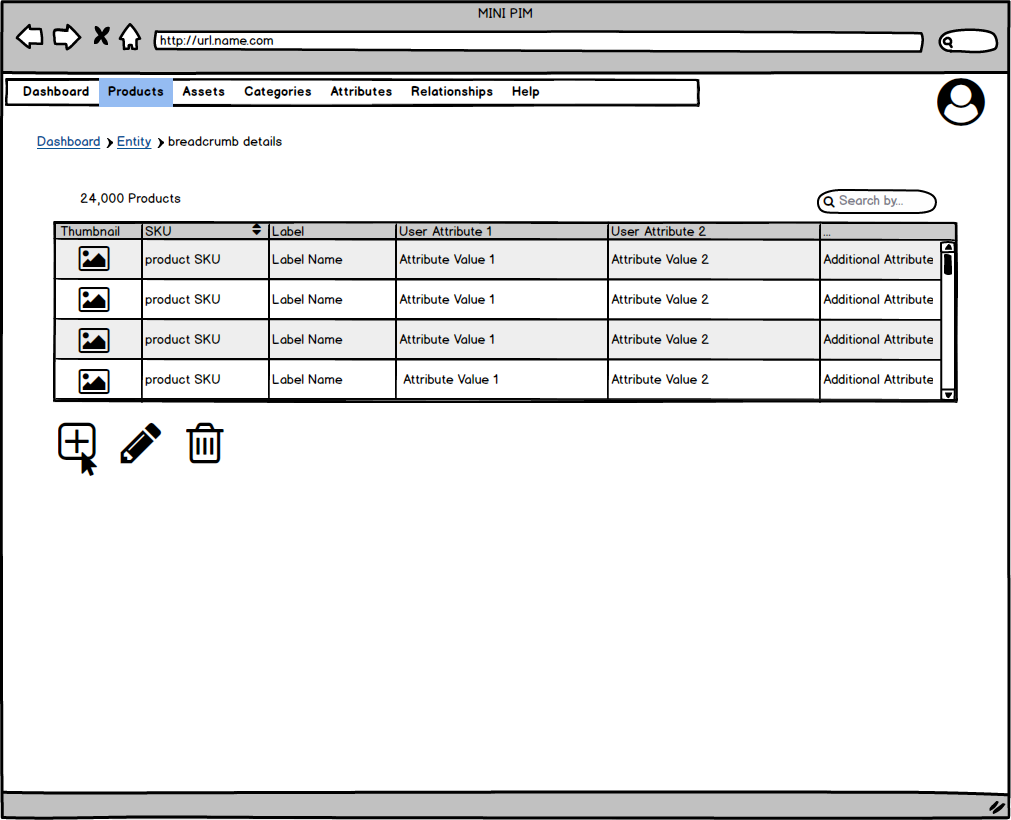
\includegraphics[width=1\linewidth]{mockups/RF2.1_boceto1.png}
    \caption{Apartado Productos hacer clic en \enquote{Añadir}}
   \end{figure}
\vspace{1.0cm}

\begin{figure}[H]
    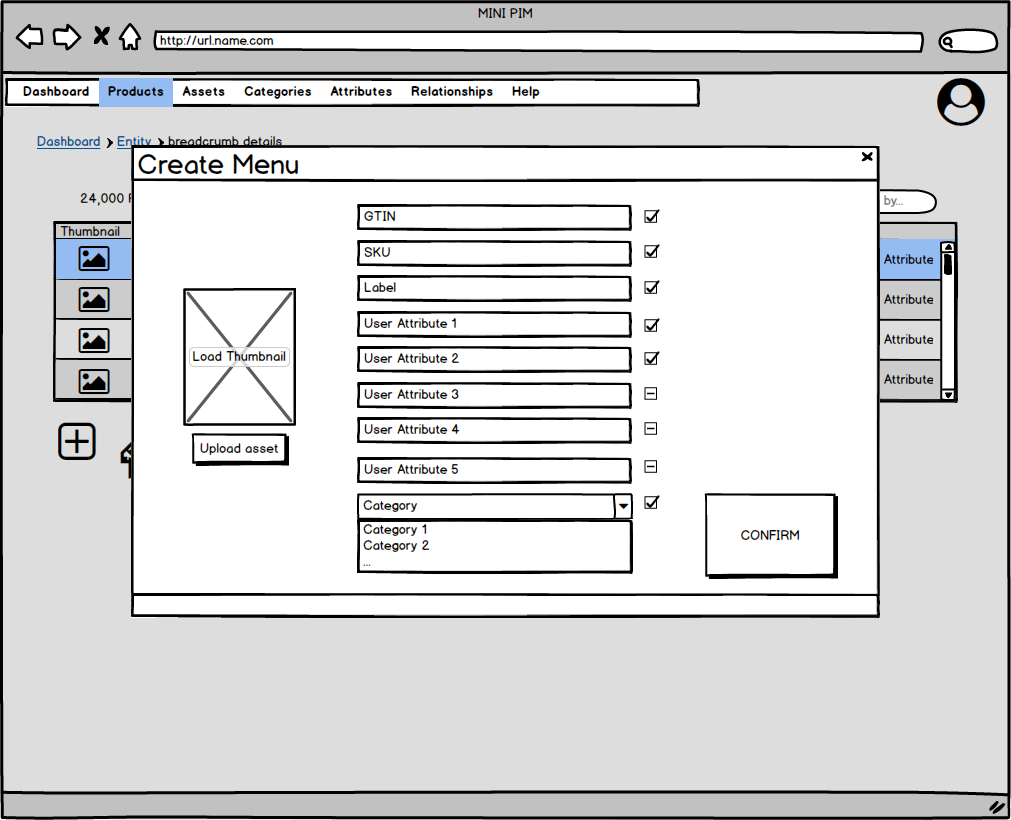
\includegraphics[width=1\linewidth]{mockups/RF2.1_bocetoCreacionV2.png}
    \caption{Menú de creación tras clicar \enquote{Añadir}}
   \end{figure}
\vspace{1.0cm}

\newpage %Inicia en una nueva página otro caso de uso
\phantomsection\numberedsection{RF2.1 Crear Producto}

\subsection*{Descripción}
Los usuarios deben de poder crear productos mientras sea posible, definiendo sus atributos y asignándoles sus respectivas categorías y relaciones.\par
\vspace{0.15cm}

\textbf{Pre-condición}\par
El usuario debe haber iniciado sesión en su cuenta en Mini PIM.\par
\vspace{0.15cm}

\textbf{Post-condición}
\begin{itemize}
    \item Caso de éxito: Todos los productos que el usuario creó se reflejan en la base de datos del sistema y en su interfaz gráfica.
    \item Caso mínimo: El sistema notifica al usuario el resultado de la acción de crear producto; exitosa o fallida.
\end{itemize}

\textbf{Prioridad: }
Alta
\vspace{0.15cm}

\textbf{Autor: }
Francisco Javier Jordá Garay\par
\vspace{0.15cm}

\textbf{Control de cambios: } Versión 1: Definición del caso de uso

\numberedsubsection{Escenario principal}
\begin{enumerate}
    \item El usuario se encuentra en el apartado de productos y selecciona la opción de \enquote{Añadir}.
    \item El sistema muestra el menú de creación solicitando al usuario:
    \begin{itemize}
        \item GTIN (atributo sistema $-$ comprueba validez de longitud)
        \item SKU (atributo sistema)
        \item Thumbnail (atributo sistema $-$ comprueba tamaño 200$\times$200px y formato)
        \item Label (atributo sistema $-$ comprueba máximo de 250 caracteres)
        \item Atributos (opcional $-$ comprueba máximo 5 nuevos atributos usuario)
        \item Categorías (opcional)
    \end{itemize}
    \item El usuario introduce los datos obligatorios y los que decida de opcionales y selecciona \enquote{Confirmar}.
    \item El sistema comprueba la validez de los datos introducidos por el usuario.
    \item El sistema almacena el producto creado en la base de datos registrando la fecha de creación.
    \item El sistema actualiza la información del total de datos registrados en la base de datos.
    \item El sistema muestra el apartado de \enquote{Productos} todos los recursos almacenados para esta sección.
\end{enumerate}

\numberedsubsection{Escenarios alternativos}
\begin{description}
    \item[2.a.] El sistema no puede almacenar el producto por superar el máximo de almacenamiento ligado al plan de suscripción del usuario.
    \begin{enumerate}
        \item[2.a.1] El sistema notifica al usuario que ha llegado al máximo de capacidad permitida en el plan de almacenamiento.
    \end{enumerate}

    \item[*.a] El usuario cancela la acción de crear un nuevo producto seleccionando la opción que cierra el menú de creación.
    \begin{enumerate}
        \item[*.a.1] El sistema regresa al apartado de \enquote{Productos}.
    \end{enumerate}

    \item[4.a] El sistema detecta un fallo en la comprobación de los datos obligatorios.
    \begin{enumerate}
        \item[4.a.1] El sistema notifica del error de comprobación al usuario mostrando el atributo del producto afectado.
        \item[4.a.2] El sistema regresa al menú de creación permitiendo edición de los datos.
    \end{enumerate}
\end{description}

\numberedsubsection{Casos de Prueba}
\underline{Escenario: Principal}\par
\vspace{0.15cm}
\textbf{Dado} que inicié sesión con mi cuenta de usuario correspondiente\par
\textbf{Y} estoy en el apartado de Productos\par
\textbf{Cuando} selecciono la opción de \enquote{Añadir}\par
\textbf{E} introduzco correctamente los atributos del producto que deseo crear\par
\textbf{Y} selecciono \enquote{confirmar} para guardar los datos\par
\textbf{Entonces} el sistema almacena la información en la base de datos de Mini PIM\par
\textbf{Y} actualiza la información del total de datos registrados en la base de datos\par
\textbf{Y} muestra el apartado de Productos con todos los recursos almacenados para esta sección.\par
\vspace{0.20cm}

\underline{Escenario: Alternativo 2.a}\par
\vspace{0.15cm}
\textbf{Dado} que inicié sesión con mi cuenta de usuario correspondiente\par
\textbf{Y} tengo el límite de productos\par
\textbf{Y} estoy en el apartado de Productos\par
\textbf{Cuando} selecciono la opción de \enquote{Añadir}\par
\textbf{E} introduzco correctamente los atributos del producto que deseo crear\par
\textbf{Y} selecciono \enquote{confirmar} para guardar los datos\par
\textbf{Entonces} el sistema me notifica que no puede almacenar el producto por superar el máximo de almacenamiento ligado a mi plan de suscripción actual\par
\vspace{0.20cm}

\underline{Escenario: Alternativo 3.a}\par
\vspace{0.15cm}
\textbf{Dado} que inicié sesión con mi cuenta de usuario correspondiente\par
\textbf{Y} estoy en el apartado de Productos\par
\textbf{Cuando} selecciono la opción de \enquote{Añadir}\par
\textbf{Y} selecciono la opción de cancelar\par
\textbf{Entonces} el sistema muestra el apartado de Productos mostrando todos los recursos almacenados sin ningún cambio.\par
\vspace{0.20cm}

\underline{Escenario: Alternativo 4.a}\par
\vspace{0.15cm}
\textbf{Dado} que inicié sesión con mi cuenta de usuario correspondiente\par
\textbf{Y} estoy en el apartado de Productos\par
\textbf{Cuando} selecciono la opción de \enquote{Añadir}\par
\textbf{Y} escribo los datos del producto y dejo uno obligatorio vacío\par
\textbf{Entonces} el sistema me muestra cual es el atributo que falla\par
\textbf{Y} regresa al menú de creación.\par
\vspace{0.20cm}

\numberedsubsection{Bocetos}
\begin{figure}[H]
    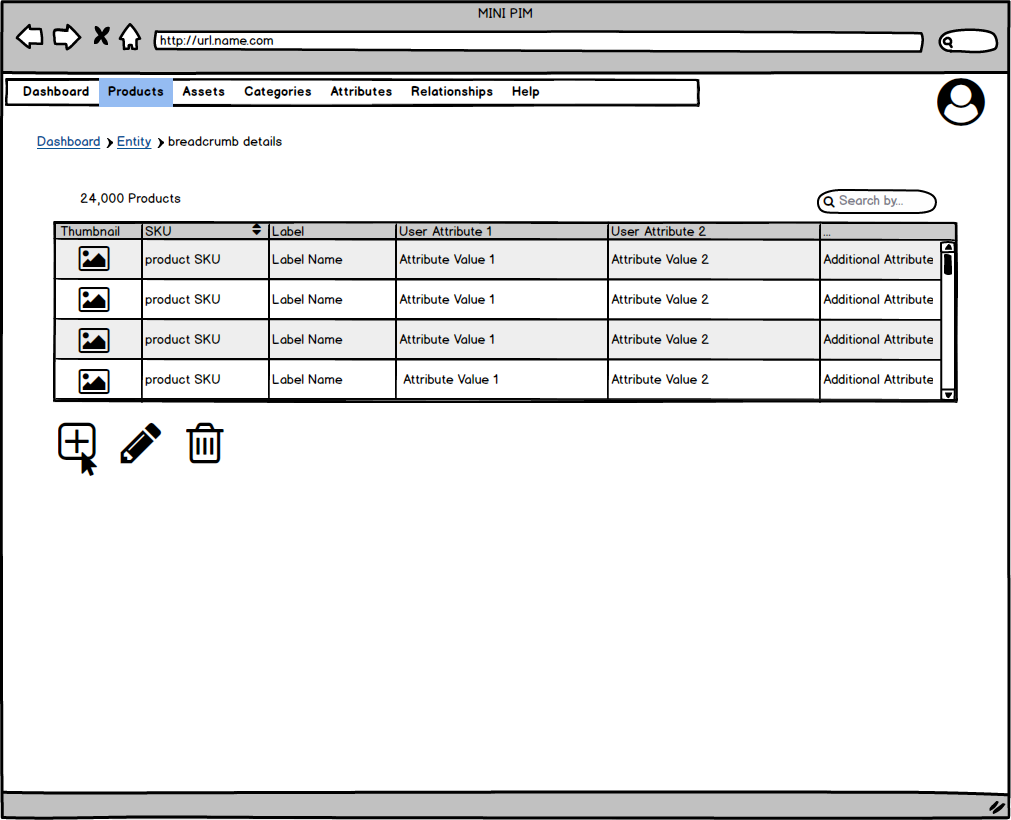
\includegraphics[width=1\linewidth]{mockups/RF2.1_boceto1.png}
    \caption{Apartado Productos hacer clic en \enquote{Añadir}}
   \end{figure}
\vspace{1.0cm}

\begin{figure}[H]
    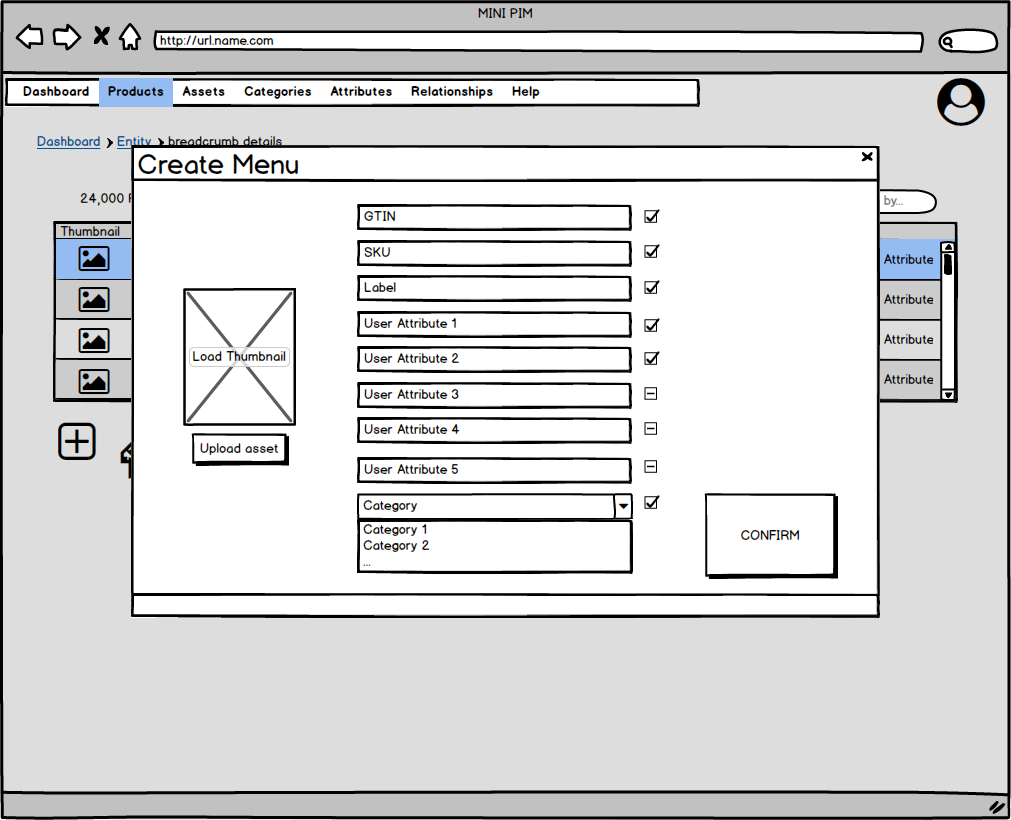
\includegraphics[width=1\linewidth]{mockups/RF2.1_bocetoCreacionV2.png}
    \caption{Menú de creación tras clicar \enquote{Añadir}}
   \end{figure}
\vspace{1.0cm}

\newpage %Inicia en una nueva página otro caso de uso
\phantomsection\numberedsection{RF2.1 Crear Producto}

\subsection*{Descripción}
Los usuarios deben de poder crear productos mientras sea posible, definiendo sus atributos y asignándoles sus respectivas categorías y relaciones.\par
\vspace{0.15cm}

\textbf{Pre-condición}\par
El usuario debe haber iniciado sesión en su cuenta en Mini PIM.\par
\vspace{0.15cm}

\textbf{Post-condición}
\begin{itemize}
    \item Caso de éxito: Todos los productos que el usuario creó se reflejan en la base de datos del sistema y en su interfaz gráfica.
    \item Caso mínimo: El sistema notifica al usuario el resultado de la acción de crear producto; exitosa o fallida.
\end{itemize}

\textbf{Prioridad: }
Alta
\vspace{0.15cm}

\textbf{Autor: }
Francisco Javier Jordá Garay\par
\vspace{0.15cm}

\textbf{Control de cambios: } Versión 1: Definición del caso de uso

\numberedsubsection{Escenario principal}
\begin{enumerate}
    \item El usuario se encuentra en el apartado de productos y selecciona la opción de \enquote{Añadir}.
    \item El sistema muestra el menú de creación solicitando al usuario:
    \begin{itemize}
        \item GTIN (atributo sistema $-$ comprueba validez de longitud)
        \item SKU (atributo sistema)
        \item Thumbnail (atributo sistema $-$ comprueba tamaño 200$\times$200px y formato)
        \item Label (atributo sistema $-$ comprueba máximo de 250 caracteres)
        \item Atributos (opcional $-$ comprueba máximo 5 nuevos atributos usuario)
        \item Categorías (opcional)
    \end{itemize}
    \item El usuario introduce los datos obligatorios y los que decida de opcionales y selecciona \enquote{Confirmar}.
    \item El sistema comprueba la validez de los datos introducidos por el usuario.
    \item El sistema almacena el producto creado en la base de datos registrando la fecha de creación.
    \item El sistema actualiza la información del total de datos registrados en la base de datos.
    \item El sistema muestra el apartado de \enquote{Productos} todos los recursos almacenados para esta sección.
\end{enumerate}

\numberedsubsection{Escenarios alternativos}
\begin{description}
    \item[2.a.] El sistema no puede almacenar el producto por superar el máximo de almacenamiento ligado al plan de suscripción del usuario.
    \begin{enumerate}
        \item[2.a.1] El sistema notifica al usuario que ha llegado al máximo de capacidad permitida en el plan de almacenamiento.
    \end{enumerate}

    \item[*.a] El usuario cancela la acción de crear un nuevo producto seleccionando la opción que cierra el menú de creación.
    \begin{enumerate}
        \item[*.a.1] El sistema regresa al apartado de \enquote{Productos}.
    \end{enumerate}

    \item[4.a] El sistema detecta un fallo en la comprobación de los datos obligatorios.
    \begin{enumerate}
        \item[4.a.1] El sistema notifica del error de comprobación al usuario mostrando el atributo del producto afectado.
        \item[4.a.2] El sistema regresa al menú de creación permitiendo edición de los datos.
    \end{enumerate}
\end{description}

\numberedsubsection{Casos de Prueba}
\underline{Escenario: Principal}\par
\vspace{0.15cm}
\textbf{Dado} que inicié sesión con mi cuenta de usuario correspondiente\par
\textbf{Y} estoy en el apartado de Productos\par
\textbf{Cuando} selecciono la opción de \enquote{Añadir}\par
\textbf{E} introduzco correctamente los atributos del producto que deseo crear\par
\textbf{Y} selecciono \enquote{confirmar} para guardar los datos\par
\textbf{Entonces} el sistema almacena la información en la base de datos de Mini PIM\par
\textbf{Y} actualiza la información del total de datos registrados en la base de datos\par
\textbf{Y} muestra el apartado de Productos con todos los recursos almacenados para esta sección.\par
\vspace{0.20cm}

\underline{Escenario: Alternativo 2.a}\par
\vspace{0.15cm}
\textbf{Dado} que inicié sesión con mi cuenta de usuario correspondiente\par
\textbf{Y} tengo el límite de productos\par
\textbf{Y} estoy en el apartado de Productos\par
\textbf{Cuando} selecciono la opción de \enquote{Añadir}\par
\textbf{E} introduzco correctamente los atributos del producto que deseo crear\par
\textbf{Y} selecciono \enquote{confirmar} para guardar los datos\par
\textbf{Entonces} el sistema me notifica que no puede almacenar el producto por superar el máximo de almacenamiento ligado a mi plan de suscripción actual\par
\vspace{0.20cm}

\underline{Escenario: Alternativo 3.a}\par
\vspace{0.15cm}
\textbf{Dado} que inicié sesión con mi cuenta de usuario correspondiente\par
\textbf{Y} estoy en el apartado de Productos\par
\textbf{Cuando} selecciono la opción de \enquote{Añadir}\par
\textbf{Y} selecciono la opción de cancelar\par
\textbf{Entonces} el sistema muestra el apartado de Productos mostrando todos los recursos almacenados sin ningún cambio.\par
\vspace{0.20cm}

\underline{Escenario: Alternativo 4.a}\par
\vspace{0.15cm}
\textbf{Dado} que inicié sesión con mi cuenta de usuario correspondiente\par
\textbf{Y} estoy en el apartado de Productos\par
\textbf{Cuando} selecciono la opción de \enquote{Añadir}\par
\textbf{Y} escribo los datos del producto y dejo uno obligatorio vacío\par
\textbf{Entonces} el sistema me muestra cual es el atributo que falla\par
\textbf{Y} regresa al menú de creación.\par
\vspace{0.20cm}

\numberedsubsection{Bocetos}
\begin{figure}[H]
    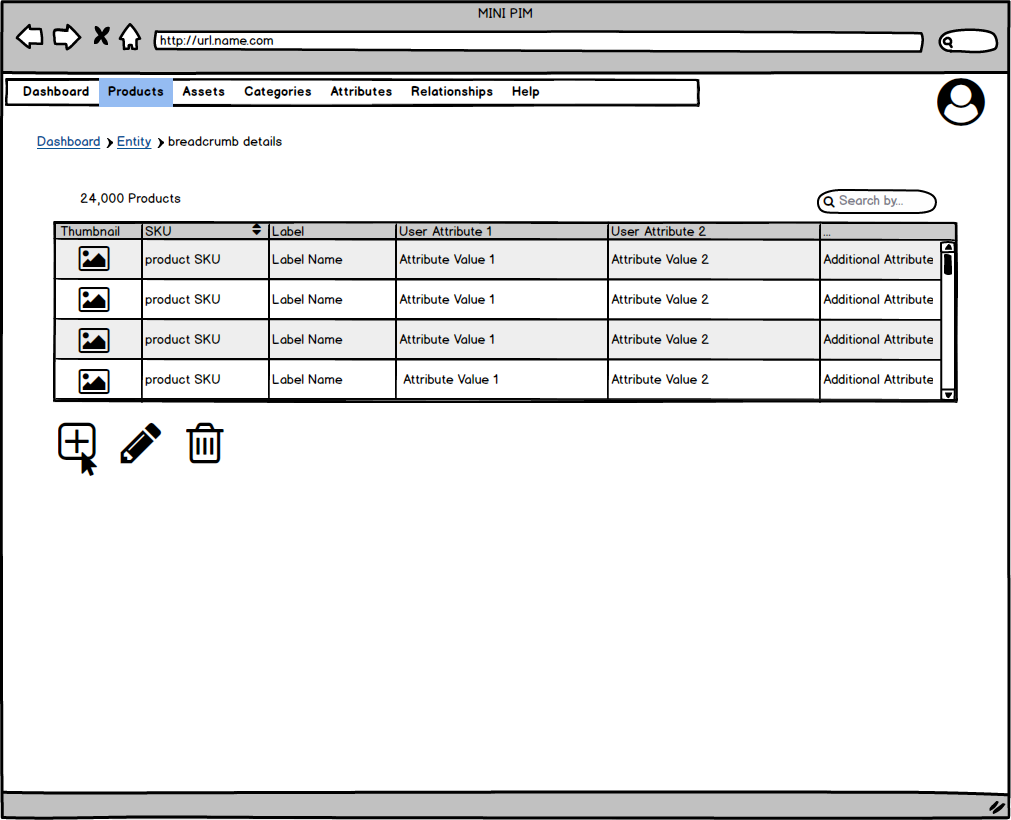
\includegraphics[width=1\linewidth]{mockups/RF2.1_boceto1.png}
    \caption{Apartado Productos hacer clic en \enquote{Añadir}}
   \end{figure}
\vspace{1.0cm}

\begin{figure}[H]
    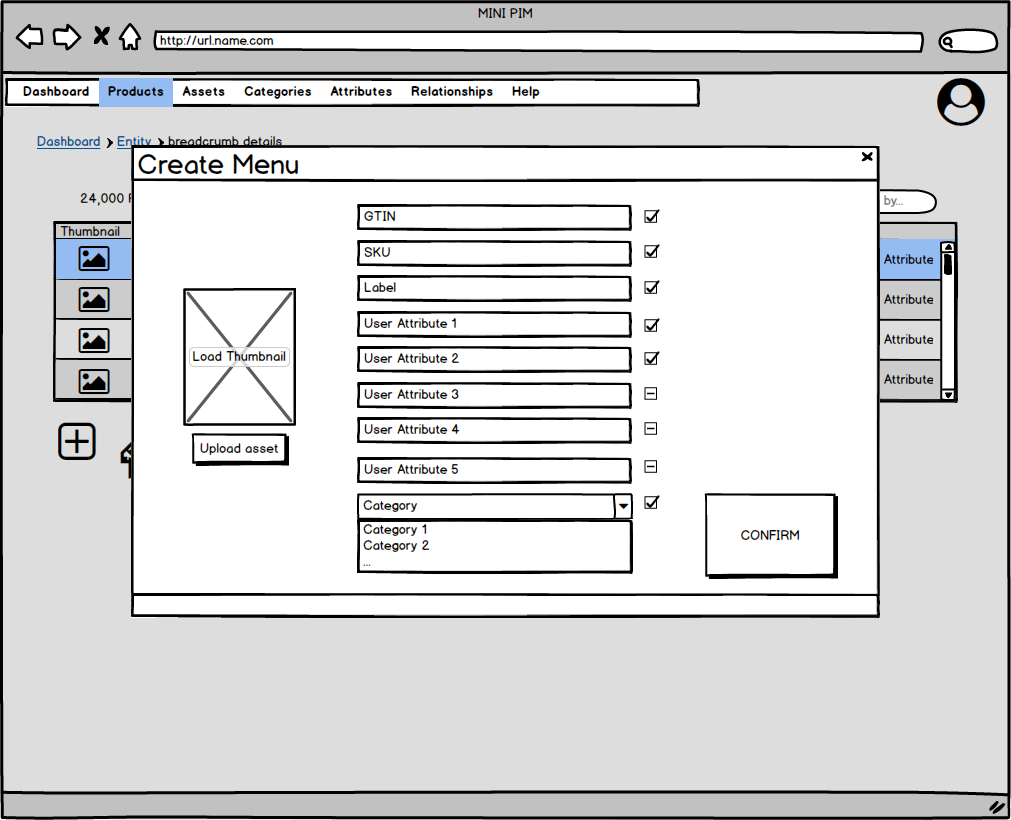
\includegraphics[width=1\linewidth]{mockups/RF2.1_bocetoCreacionV2.png}
    \caption{Menú de creación tras clicar \enquote{Añadir}}
   \end{figure}
\vspace{1.0cm}

\newpage %Inicia en una nueva página otro caso de uso
\phantomsection\numberedsection{RF2.1 Crear Producto}

\subsection*{Descripción}
Los usuarios deben de poder crear productos mientras sea posible, definiendo sus atributos y asignándoles sus respectivas categorías y relaciones.\par
\vspace{0.15cm}

\textbf{Pre-condición}\par
El usuario debe haber iniciado sesión en su cuenta en Mini PIM.\par
\vspace{0.15cm}

\textbf{Post-condición}
\begin{itemize}
    \item Caso de éxito: Todos los productos que el usuario creó se reflejan en la base de datos del sistema y en su interfaz gráfica.
    \item Caso mínimo: El sistema notifica al usuario el resultado de la acción de crear producto; exitosa o fallida.
\end{itemize}

\textbf{Prioridad: }
Alta
\vspace{0.15cm}

\textbf{Autor: }
Francisco Javier Jordá Garay\par
\vspace{0.15cm}

\textbf{Control de cambios: } Versión 1: Definición del caso de uso

\numberedsubsection{Escenario principal}
\begin{enumerate}
    \item El usuario se encuentra en el apartado de productos y selecciona la opción de \enquote{Añadir}.
    \item El sistema muestra el menú de creación solicitando al usuario:
    \begin{itemize}
        \item GTIN (atributo sistema $-$ comprueba validez de longitud)
        \item SKU (atributo sistema)
        \item Thumbnail (atributo sistema $-$ comprueba tamaño 200$\times$200px y formato)
        \item Label (atributo sistema $-$ comprueba máximo de 250 caracteres)
        \item Atributos (opcional $-$ comprueba máximo 5 nuevos atributos usuario)
        \item Categorías (opcional)
    \end{itemize}
    \item El usuario introduce los datos obligatorios y los que decida de opcionales y selecciona \enquote{Confirmar}.
    \item El sistema comprueba la validez de los datos introducidos por el usuario.
    \item El sistema almacena el producto creado en la base de datos registrando la fecha de creación.
    \item El sistema actualiza la información del total de datos registrados en la base de datos.
    \item El sistema muestra el apartado de \enquote{Productos} todos los recursos almacenados para esta sección.
\end{enumerate}

\numberedsubsection{Escenarios alternativos}
\begin{description}
    \item[2.a.] El sistema no puede almacenar el producto por superar el máximo de almacenamiento ligado al plan de suscripción del usuario.
    \begin{enumerate}
        \item[2.a.1] El sistema notifica al usuario que ha llegado al máximo de capacidad permitida en el plan de almacenamiento.
    \end{enumerate}

    \item[*.a] El usuario cancela la acción de crear un nuevo producto seleccionando la opción que cierra el menú de creación.
    \begin{enumerate}
        \item[*.a.1] El sistema regresa al apartado de \enquote{Productos}.
    \end{enumerate}

    \item[4.a] El sistema detecta un fallo en la comprobación de los datos obligatorios.
    \begin{enumerate}
        \item[4.a.1] El sistema notifica del error de comprobación al usuario mostrando el atributo del producto afectado.
        \item[4.a.2] El sistema regresa al menú de creación permitiendo edición de los datos.
    \end{enumerate}
\end{description}

\numberedsubsection{Casos de Prueba}
\underline{Escenario: Principal}\par
\vspace{0.15cm}
\textbf{Dado} que inicié sesión con mi cuenta de usuario correspondiente\par
\textbf{Y} estoy en el apartado de Productos\par
\textbf{Cuando} selecciono la opción de \enquote{Añadir}\par
\textbf{E} introduzco correctamente los atributos del producto que deseo crear\par
\textbf{Y} selecciono \enquote{confirmar} para guardar los datos\par
\textbf{Entonces} el sistema almacena la información en la base de datos de Mini PIM\par
\textbf{Y} actualiza la información del total de datos registrados en la base de datos\par
\textbf{Y} muestra el apartado de Productos con todos los recursos almacenados para esta sección.\par
\vspace{0.20cm}

\underline{Escenario: Alternativo 2.a}\par
\vspace{0.15cm}
\textbf{Dado} que inicié sesión con mi cuenta de usuario correspondiente\par
\textbf{Y} tengo el límite de productos\par
\textbf{Y} estoy en el apartado de Productos\par
\textbf{Cuando} selecciono la opción de \enquote{Añadir}\par
\textbf{E} introduzco correctamente los atributos del producto que deseo crear\par
\textbf{Y} selecciono \enquote{confirmar} para guardar los datos\par
\textbf{Entonces} el sistema me notifica que no puede almacenar el producto por superar el máximo de almacenamiento ligado a mi plan de suscripción actual\par
\vspace{0.20cm}

\underline{Escenario: Alternativo 3.a}\par
\vspace{0.15cm}
\textbf{Dado} que inicié sesión con mi cuenta de usuario correspondiente\par
\textbf{Y} estoy en el apartado de Productos\par
\textbf{Cuando} selecciono la opción de \enquote{Añadir}\par
\textbf{Y} selecciono la opción de cancelar\par
\textbf{Entonces} el sistema muestra el apartado de Productos mostrando todos los recursos almacenados sin ningún cambio.\par
\vspace{0.20cm}

\underline{Escenario: Alternativo 4.a}\par
\vspace{0.15cm}
\textbf{Dado} que inicié sesión con mi cuenta de usuario correspondiente\par
\textbf{Y} estoy en el apartado de Productos\par
\textbf{Cuando} selecciono la opción de \enquote{Añadir}\par
\textbf{Y} escribo los datos del producto y dejo uno obligatorio vacío\par
\textbf{Entonces} el sistema me muestra cual es el atributo que falla\par
\textbf{Y} regresa al menú de creación.\par
\vspace{0.20cm}

\numberedsubsection{Bocetos}
\begin{figure}[H]
    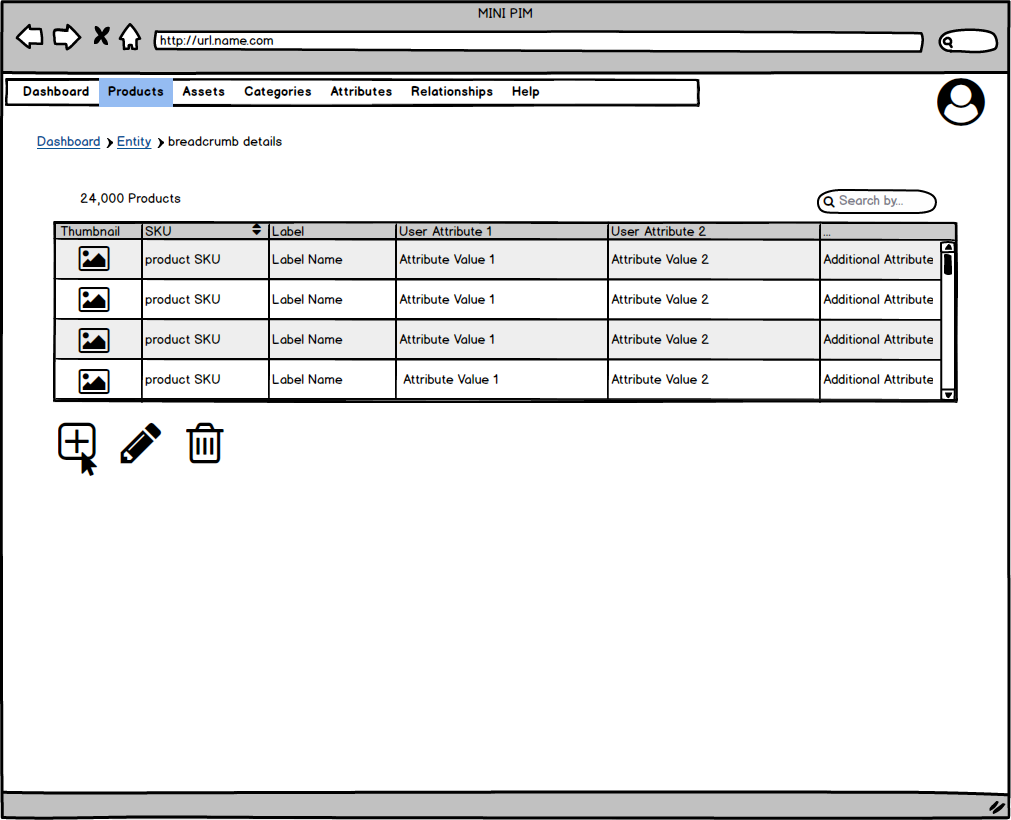
\includegraphics[width=1\linewidth]{mockups/RF2.1_boceto1.png}
    \caption{Apartado Productos hacer clic en \enquote{Añadir}}
   \end{figure}
\vspace{1.0cm}

\begin{figure}[H]
    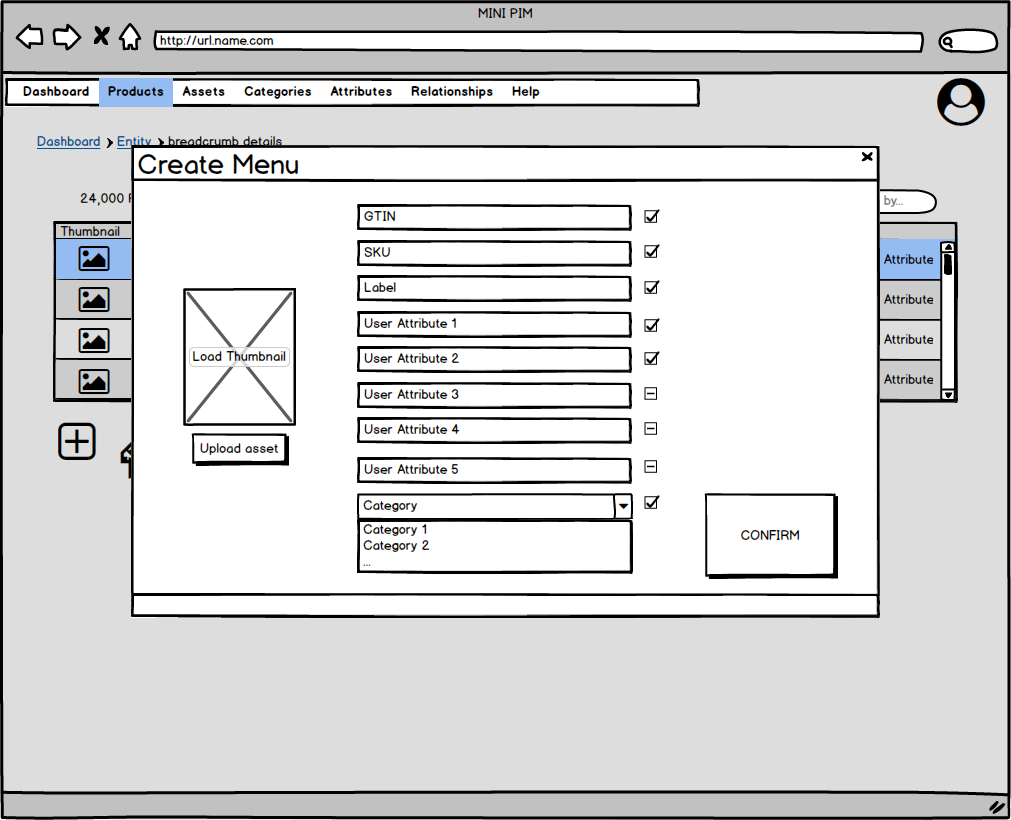
\includegraphics[width=1\linewidth]{mockups/RF2.1_bocetoCreacionV2.png}
    \caption{Menú de creación tras clicar \enquote{Añadir}}
   \end{figure}
\vspace{1.0cm}

\newpage %Inicia en una nueva página otro caso de uso
\phantomsection\numberedsection{RF2.1 Crear Producto}

\subsection*{Descripción}
Los usuarios deben de poder crear productos mientras sea posible, definiendo sus atributos y asignándoles sus respectivas categorías y relaciones.\par
\vspace{0.15cm}

\textbf{Pre-condición}\par
El usuario debe haber iniciado sesión en su cuenta en Mini PIM.\par
\vspace{0.15cm}

\textbf{Post-condición}
\begin{itemize}
    \item Caso de éxito: Todos los productos que el usuario creó se reflejan en la base de datos del sistema y en su interfaz gráfica.
    \item Caso mínimo: El sistema notifica al usuario el resultado de la acción de crear producto; exitosa o fallida.
\end{itemize}

\textbf{Prioridad: }
Alta
\vspace{0.15cm}

\textbf{Autor: }
Francisco Javier Jordá Garay\par
\vspace{0.15cm}

\textbf{Control de cambios: } Versión 1: Definición del caso de uso

\numberedsubsection{Escenario principal}
\begin{enumerate}
    \item El usuario se encuentra en el apartado de productos y selecciona la opción de \enquote{Añadir}.
    \item El sistema muestra el menú de creación solicitando al usuario:
    \begin{itemize}
        \item GTIN (atributo sistema $-$ comprueba validez de longitud)
        \item SKU (atributo sistema)
        \item Thumbnail (atributo sistema $-$ comprueba tamaño 200$\times$200px y formato)
        \item Label (atributo sistema $-$ comprueba máximo de 250 caracteres)
        \item Atributos (opcional $-$ comprueba máximo 5 nuevos atributos usuario)
        \item Categorías (opcional)
    \end{itemize}
    \item El usuario introduce los datos obligatorios y los que decida de opcionales y selecciona \enquote{Confirmar}.
    \item El sistema comprueba la validez de los datos introducidos por el usuario.
    \item El sistema almacena el producto creado en la base de datos registrando la fecha de creación.
    \item El sistema actualiza la información del total de datos registrados en la base de datos.
    \item El sistema muestra el apartado de \enquote{Productos} todos los recursos almacenados para esta sección.
\end{enumerate}

\numberedsubsection{Escenarios alternativos}
\begin{description}
    \item[2.a.] El sistema no puede almacenar el producto por superar el máximo de almacenamiento ligado al plan de suscripción del usuario.
    \begin{enumerate}
        \item[2.a.1] El sistema notifica al usuario que ha llegado al máximo de capacidad permitida en el plan de almacenamiento.
    \end{enumerate}

    \item[*.a] El usuario cancela la acción de crear un nuevo producto seleccionando la opción que cierra el menú de creación.
    \begin{enumerate}
        \item[*.a.1] El sistema regresa al apartado de \enquote{Productos}.
    \end{enumerate}

    \item[4.a] El sistema detecta un fallo en la comprobación de los datos obligatorios.
    \begin{enumerate}
        \item[4.a.1] El sistema notifica del error de comprobación al usuario mostrando el atributo del producto afectado.
        \item[4.a.2] El sistema regresa al menú de creación permitiendo edición de los datos.
    \end{enumerate}
\end{description}

\numberedsubsection{Casos de Prueba}
\underline{Escenario: Principal}\par
\vspace{0.15cm}
\textbf{Dado} que inicié sesión con mi cuenta de usuario correspondiente\par
\textbf{Y} estoy en el apartado de Productos\par
\textbf{Cuando} selecciono la opción de \enquote{Añadir}\par
\textbf{E} introduzco correctamente los atributos del producto que deseo crear\par
\textbf{Y} selecciono \enquote{confirmar} para guardar los datos\par
\textbf{Entonces} el sistema almacena la información en la base de datos de Mini PIM\par
\textbf{Y} actualiza la información del total de datos registrados en la base de datos\par
\textbf{Y} muestra el apartado de Productos con todos los recursos almacenados para esta sección.\par
\vspace{0.20cm}

\underline{Escenario: Alternativo 2.a}\par
\vspace{0.15cm}
\textbf{Dado} que inicié sesión con mi cuenta de usuario correspondiente\par
\textbf{Y} tengo el límite de productos\par
\textbf{Y} estoy en el apartado de Productos\par
\textbf{Cuando} selecciono la opción de \enquote{Añadir}\par
\textbf{E} introduzco correctamente los atributos del producto que deseo crear\par
\textbf{Y} selecciono \enquote{confirmar} para guardar los datos\par
\textbf{Entonces} el sistema me notifica que no puede almacenar el producto por superar el máximo de almacenamiento ligado a mi plan de suscripción actual\par
\vspace{0.20cm}

\underline{Escenario: Alternativo 3.a}\par
\vspace{0.15cm}
\textbf{Dado} que inicié sesión con mi cuenta de usuario correspondiente\par
\textbf{Y} estoy en el apartado de Productos\par
\textbf{Cuando} selecciono la opción de \enquote{Añadir}\par
\textbf{Y} selecciono la opción de cancelar\par
\textbf{Entonces} el sistema muestra el apartado de Productos mostrando todos los recursos almacenados sin ningún cambio.\par
\vspace{0.20cm}

\underline{Escenario: Alternativo 4.a}\par
\vspace{0.15cm}
\textbf{Dado} que inicié sesión con mi cuenta de usuario correspondiente\par
\textbf{Y} estoy en el apartado de Productos\par
\textbf{Cuando} selecciono la opción de \enquote{Añadir}\par
\textbf{Y} escribo los datos del producto y dejo uno obligatorio vacío\par
\textbf{Entonces} el sistema me muestra cual es el atributo que falla\par
\textbf{Y} regresa al menú de creación.\par
\vspace{0.20cm}

\numberedsubsection{Bocetos}
\begin{figure}[H]
    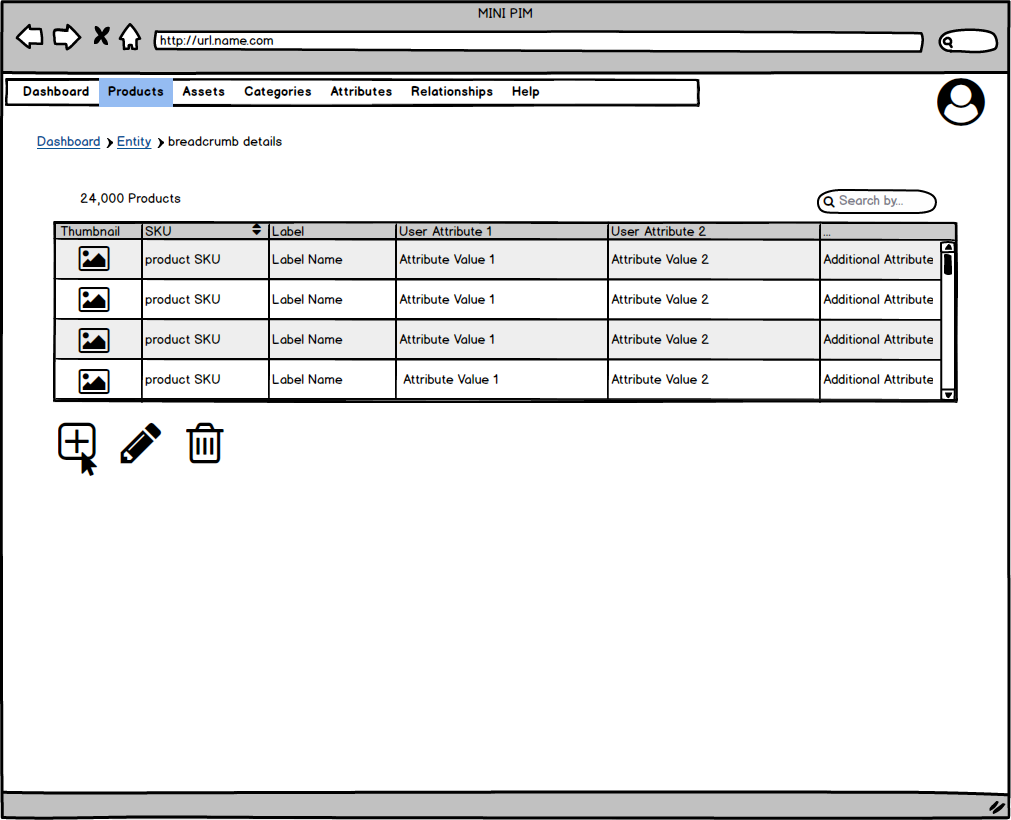
\includegraphics[width=1\linewidth]{mockups/RF2.1_boceto1.png}
    \caption{Apartado Productos hacer clic en \enquote{Añadir}}
   \end{figure}
\vspace{1.0cm}

\begin{figure}[H]
    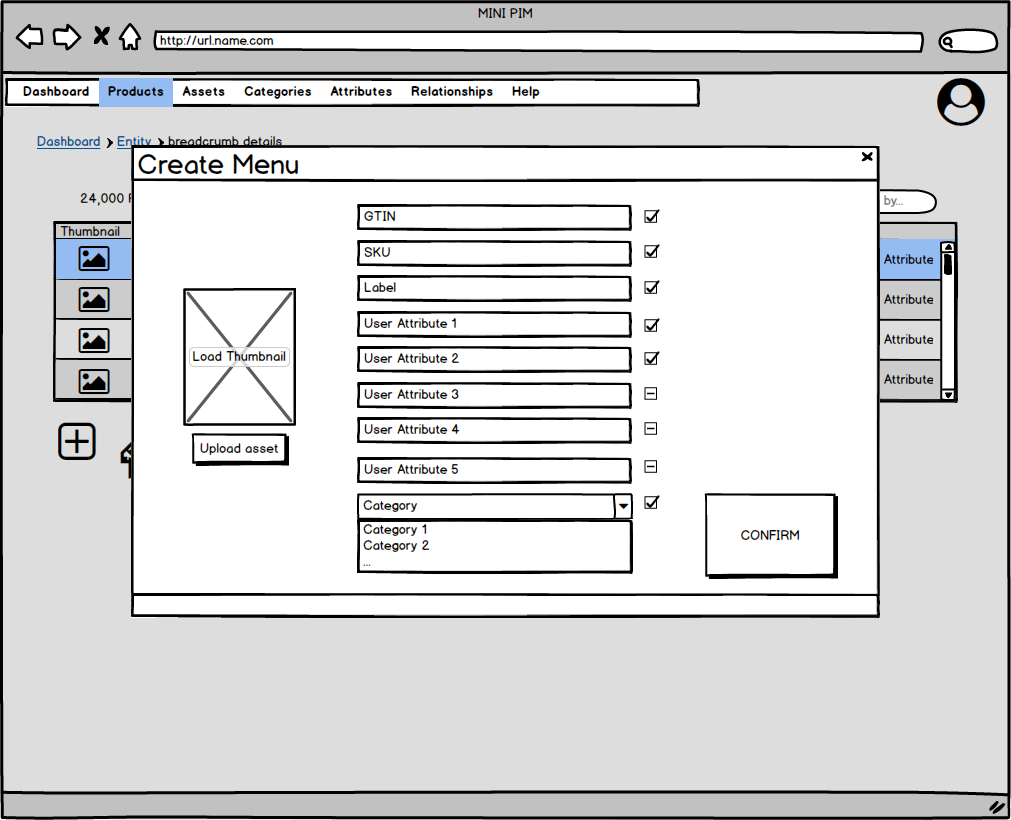
\includegraphics[width=1\linewidth]{mockups/RF2.1_bocetoCreacionV2.png}
    \caption{Menú de creación tras clicar \enquote{Añadir}}
   \end{figure}
\vspace{1.0cm}

\newpage %Inicia en una nueva página otro caso de uso
\phantomsection\numberedsection{RF2.1 Crear Producto}

\subsection*{Descripción}
Los usuarios deben de poder crear productos mientras sea posible, definiendo sus atributos y asignándoles sus respectivas categorías y relaciones.\par
\vspace{0.15cm}

\textbf{Pre-condición}\par
El usuario debe haber iniciado sesión en su cuenta en Mini PIM.\par
\vspace{0.15cm}

\textbf{Post-condición}
\begin{itemize}
    \item Caso de éxito: Todos los productos que el usuario creó se reflejan en la base de datos del sistema y en su interfaz gráfica.
    \item Caso mínimo: El sistema notifica al usuario el resultado de la acción de crear producto; exitosa o fallida.
\end{itemize}

\textbf{Prioridad: }
Alta
\vspace{0.15cm}

\textbf{Autor: }
Francisco Javier Jordá Garay\par
\vspace{0.15cm}

\textbf{Control de cambios: } Versión 1: Definición del caso de uso

\numberedsubsection{Escenario principal}
\begin{enumerate}
    \item El usuario se encuentra en el apartado de productos y selecciona la opción de \enquote{Añadir}.
    \item El sistema muestra el menú de creación solicitando al usuario:
    \begin{itemize}
        \item GTIN (atributo sistema $-$ comprueba validez de longitud)
        \item SKU (atributo sistema)
        \item Thumbnail (atributo sistema $-$ comprueba tamaño 200$\times$200px y formato)
        \item Label (atributo sistema $-$ comprueba máximo de 250 caracteres)
        \item Atributos (opcional $-$ comprueba máximo 5 nuevos atributos usuario)
        \item Categorías (opcional)
    \end{itemize}
    \item El usuario introduce los datos obligatorios y los que decida de opcionales y selecciona \enquote{Confirmar}.
    \item El sistema comprueba la validez de los datos introducidos por el usuario.
    \item El sistema almacena el producto creado en la base de datos registrando la fecha de creación.
    \item El sistema actualiza la información del total de datos registrados en la base de datos.
    \item El sistema muestra el apartado de \enquote{Productos} todos los recursos almacenados para esta sección.
\end{enumerate}

\numberedsubsection{Escenarios alternativos}
\begin{description}
    \item[2.a.] El sistema no puede almacenar el producto por superar el máximo de almacenamiento ligado al plan de suscripción del usuario.
    \begin{enumerate}
        \item[2.a.1] El sistema notifica al usuario que ha llegado al máximo de capacidad permitida en el plan de almacenamiento.
    \end{enumerate}

    \item[*.a] El usuario cancela la acción de crear un nuevo producto seleccionando la opción que cierra el menú de creación.
    \begin{enumerate}
        \item[*.a.1] El sistema regresa al apartado de \enquote{Productos}.
    \end{enumerate}

    \item[4.a] El sistema detecta un fallo en la comprobación de los datos obligatorios.
    \begin{enumerate}
        \item[4.a.1] El sistema notifica del error de comprobación al usuario mostrando el atributo del producto afectado.
        \item[4.a.2] El sistema regresa al menú de creación permitiendo edición de los datos.
    \end{enumerate}
\end{description}

\numberedsubsection{Casos de Prueba}
\underline{Escenario: Principal}\par
\vspace{0.15cm}
\textbf{Dado} que inicié sesión con mi cuenta de usuario correspondiente\par
\textbf{Y} estoy en el apartado de Productos\par
\textbf{Cuando} selecciono la opción de \enquote{Añadir}\par
\textbf{E} introduzco correctamente los atributos del producto que deseo crear\par
\textbf{Y} selecciono \enquote{confirmar} para guardar los datos\par
\textbf{Entonces} el sistema almacena la información en la base de datos de Mini PIM\par
\textbf{Y} actualiza la información del total de datos registrados en la base de datos\par
\textbf{Y} muestra el apartado de Productos con todos los recursos almacenados para esta sección.\par
\vspace{0.20cm}

\underline{Escenario: Alternativo 2.a}\par
\vspace{0.15cm}
\textbf{Dado} que inicié sesión con mi cuenta de usuario correspondiente\par
\textbf{Y} tengo el límite de productos\par
\textbf{Y} estoy en el apartado de Productos\par
\textbf{Cuando} selecciono la opción de \enquote{Añadir}\par
\textbf{E} introduzco correctamente los atributos del producto que deseo crear\par
\textbf{Y} selecciono \enquote{confirmar} para guardar los datos\par
\textbf{Entonces} el sistema me notifica que no puede almacenar el producto por superar el máximo de almacenamiento ligado a mi plan de suscripción actual\par
\vspace{0.20cm}

\underline{Escenario: Alternativo 3.a}\par
\vspace{0.15cm}
\textbf{Dado} que inicié sesión con mi cuenta de usuario correspondiente\par
\textbf{Y} estoy en el apartado de Productos\par
\textbf{Cuando} selecciono la opción de \enquote{Añadir}\par
\textbf{Y} selecciono la opción de cancelar\par
\textbf{Entonces} el sistema muestra el apartado de Productos mostrando todos los recursos almacenados sin ningún cambio.\par
\vspace{0.20cm}

\underline{Escenario: Alternativo 4.a}\par
\vspace{0.15cm}
\textbf{Dado} que inicié sesión con mi cuenta de usuario correspondiente\par
\textbf{Y} estoy en el apartado de Productos\par
\textbf{Cuando} selecciono la opción de \enquote{Añadir}\par
\textbf{Y} escribo los datos del producto y dejo uno obligatorio vacío\par
\textbf{Entonces} el sistema me muestra cual es el atributo que falla\par
\textbf{Y} regresa al menú de creación.\par
\vspace{0.20cm}

\numberedsubsection{Bocetos}
\begin{figure}[H]
    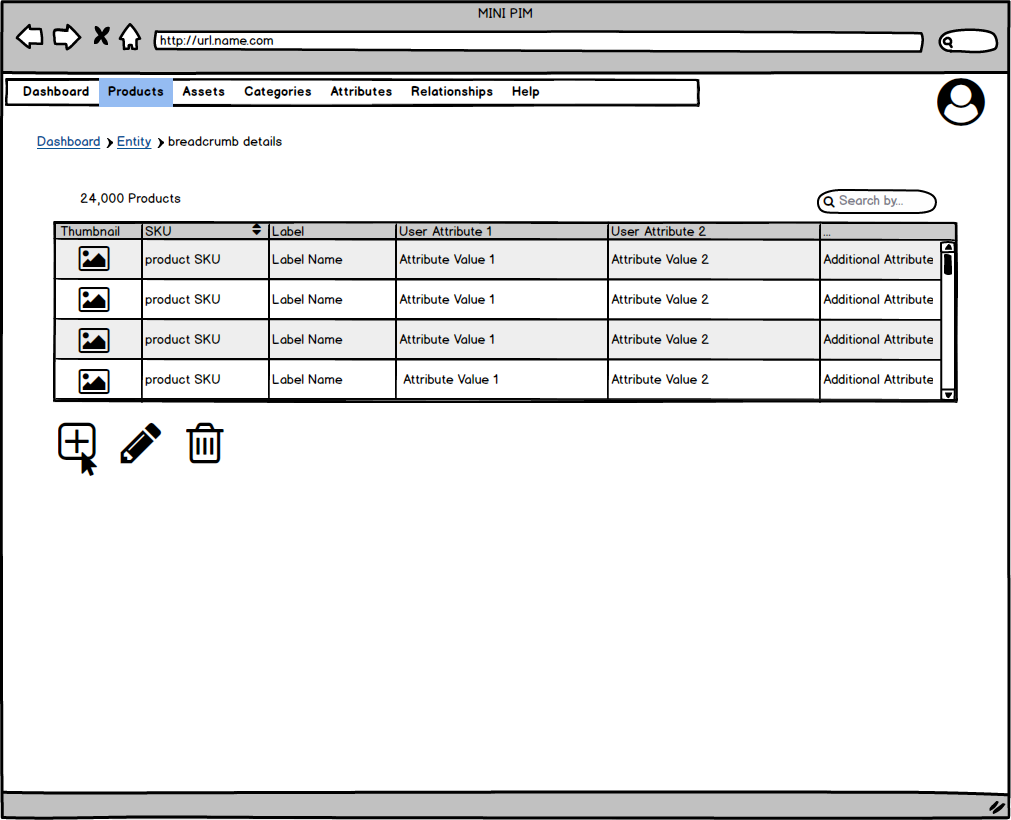
\includegraphics[width=1\linewidth]{mockups/RF2.1_boceto1.png}
    \caption{Apartado Productos hacer clic en \enquote{Añadir}}
   \end{figure}
\vspace{1.0cm}

\begin{figure}[H]
    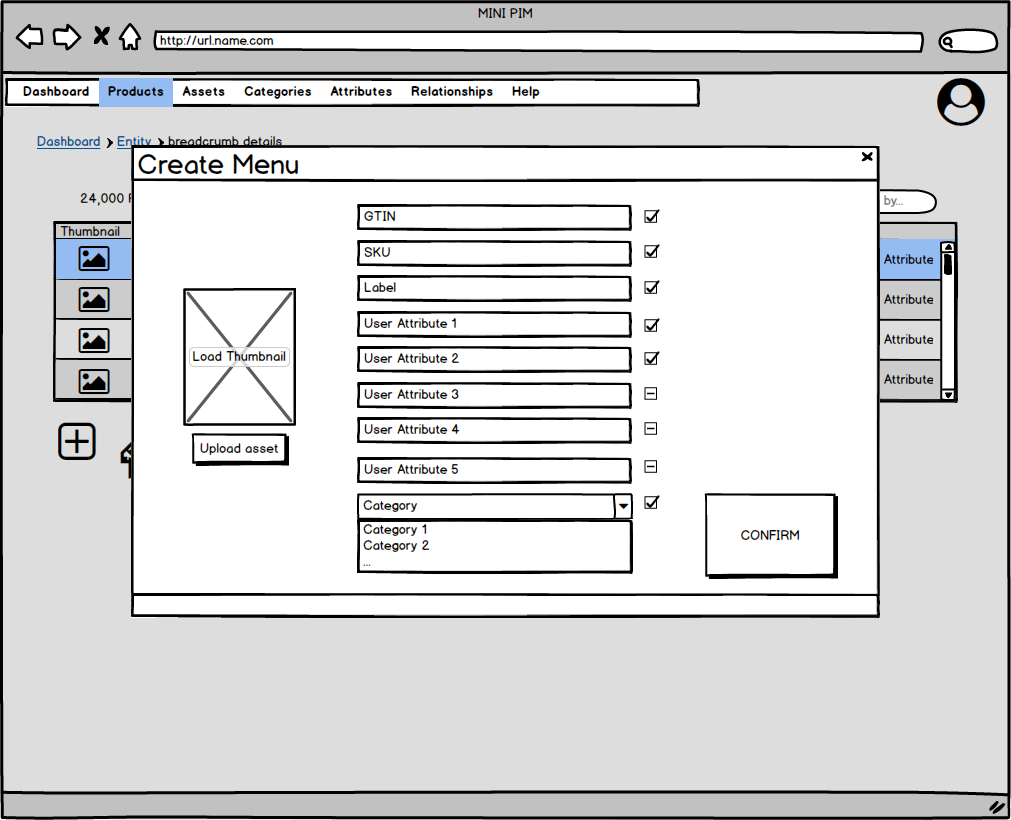
\includegraphics[width=1\linewidth]{mockups/RF2.1_bocetoCreacionV2.png}
    \caption{Menú de creación tras clicar \enquote{Añadir}}
   \end{figure}
\vspace{1.0cm}

\newpage %Inicia en una nueva página otro caso de uso
\phantomsection\numberedsection{RF2.1 Crear Producto}

\subsection*{Descripción}
Los usuarios deben de poder crear productos mientras sea posible, definiendo sus atributos y asignándoles sus respectivas categorías y relaciones.\par
\vspace{0.15cm}

\textbf{Pre-condición}\par
El usuario debe haber iniciado sesión en su cuenta en Mini PIM.\par
\vspace{0.15cm}

\textbf{Post-condición}
\begin{itemize}
    \item Caso de éxito: Todos los productos que el usuario creó se reflejan en la base de datos del sistema y en su interfaz gráfica.
    \item Caso mínimo: El sistema notifica al usuario el resultado de la acción de crear producto; exitosa o fallida.
\end{itemize}

\textbf{Prioridad: }
Alta
\vspace{0.15cm}

\textbf{Autor: }
Francisco Javier Jordá Garay\par
\vspace{0.15cm}

\textbf{Control de cambios: } Versión 1: Definición del caso de uso

\numberedsubsection{Escenario principal}
\begin{enumerate}
    \item El usuario se encuentra en el apartado de productos y selecciona la opción de \enquote{Añadir}.
    \item El sistema muestra el menú de creación solicitando al usuario:
    \begin{itemize}
        \item GTIN (atributo sistema $-$ comprueba validez de longitud)
        \item SKU (atributo sistema)
        \item Thumbnail (atributo sistema $-$ comprueba tamaño 200$\times$200px y formato)
        \item Label (atributo sistema $-$ comprueba máximo de 250 caracteres)
        \item Atributos (opcional $-$ comprueba máximo 5 nuevos atributos usuario)
        \item Categorías (opcional)
    \end{itemize}
    \item El usuario introduce los datos obligatorios y los que decida de opcionales y selecciona \enquote{Confirmar}.
    \item El sistema comprueba la validez de los datos introducidos por el usuario.
    \item El sistema almacena el producto creado en la base de datos registrando la fecha de creación.
    \item El sistema actualiza la información del total de datos registrados en la base de datos.
    \item El sistema muestra el apartado de \enquote{Productos} todos los recursos almacenados para esta sección.
\end{enumerate}

\numberedsubsection{Escenarios alternativos}
\begin{description}
    \item[2.a.] El sistema no puede almacenar el producto por superar el máximo de almacenamiento ligado al plan de suscripción del usuario.
    \begin{enumerate}
        \item[2.a.1] El sistema notifica al usuario que ha llegado al máximo de capacidad permitida en el plan de almacenamiento.
    \end{enumerate}

    \item[*.a] El usuario cancela la acción de crear un nuevo producto seleccionando la opción que cierra el menú de creación.
    \begin{enumerate}
        \item[*.a.1] El sistema regresa al apartado de \enquote{Productos}.
    \end{enumerate}

    \item[4.a] El sistema detecta un fallo en la comprobación de los datos obligatorios.
    \begin{enumerate}
        \item[4.a.1] El sistema notifica del error de comprobación al usuario mostrando el atributo del producto afectado.
        \item[4.a.2] El sistema regresa al menú de creación permitiendo edición de los datos.
    \end{enumerate}
\end{description}

\numberedsubsection{Casos de Prueba}
\underline{Escenario: Principal}\par
\vspace{0.15cm}
\textbf{Dado} que inicié sesión con mi cuenta de usuario correspondiente\par
\textbf{Y} estoy en el apartado de Productos\par
\textbf{Cuando} selecciono la opción de \enquote{Añadir}\par
\textbf{E} introduzco correctamente los atributos del producto que deseo crear\par
\textbf{Y} selecciono \enquote{confirmar} para guardar los datos\par
\textbf{Entonces} el sistema almacena la información en la base de datos de Mini PIM\par
\textbf{Y} actualiza la información del total de datos registrados en la base de datos\par
\textbf{Y} muestra el apartado de Productos con todos los recursos almacenados para esta sección.\par
\vspace{0.20cm}

\underline{Escenario: Alternativo 2.a}\par
\vspace{0.15cm}
\textbf{Dado} que inicié sesión con mi cuenta de usuario correspondiente\par
\textbf{Y} tengo el límite de productos\par
\textbf{Y} estoy en el apartado de Productos\par
\textbf{Cuando} selecciono la opción de \enquote{Añadir}\par
\textbf{E} introduzco correctamente los atributos del producto que deseo crear\par
\textbf{Y} selecciono \enquote{confirmar} para guardar los datos\par
\textbf{Entonces} el sistema me notifica que no puede almacenar el producto por superar el máximo de almacenamiento ligado a mi plan de suscripción actual\par
\vspace{0.20cm}

\underline{Escenario: Alternativo 3.a}\par
\vspace{0.15cm}
\textbf{Dado} que inicié sesión con mi cuenta de usuario correspondiente\par
\textbf{Y} estoy en el apartado de Productos\par
\textbf{Cuando} selecciono la opción de \enquote{Añadir}\par
\textbf{Y} selecciono la opción de cancelar\par
\textbf{Entonces} el sistema muestra el apartado de Productos mostrando todos los recursos almacenados sin ningún cambio.\par
\vspace{0.20cm}

\underline{Escenario: Alternativo 4.a}\par
\vspace{0.15cm}
\textbf{Dado} que inicié sesión con mi cuenta de usuario correspondiente\par
\textbf{Y} estoy en el apartado de Productos\par
\textbf{Cuando} selecciono la opción de \enquote{Añadir}\par
\textbf{Y} escribo los datos del producto y dejo uno obligatorio vacío\par
\textbf{Entonces} el sistema me muestra cual es el atributo que falla\par
\textbf{Y} regresa al menú de creación.\par
\vspace{0.20cm}

\numberedsubsection{Bocetos}
\begin{figure}[H]
    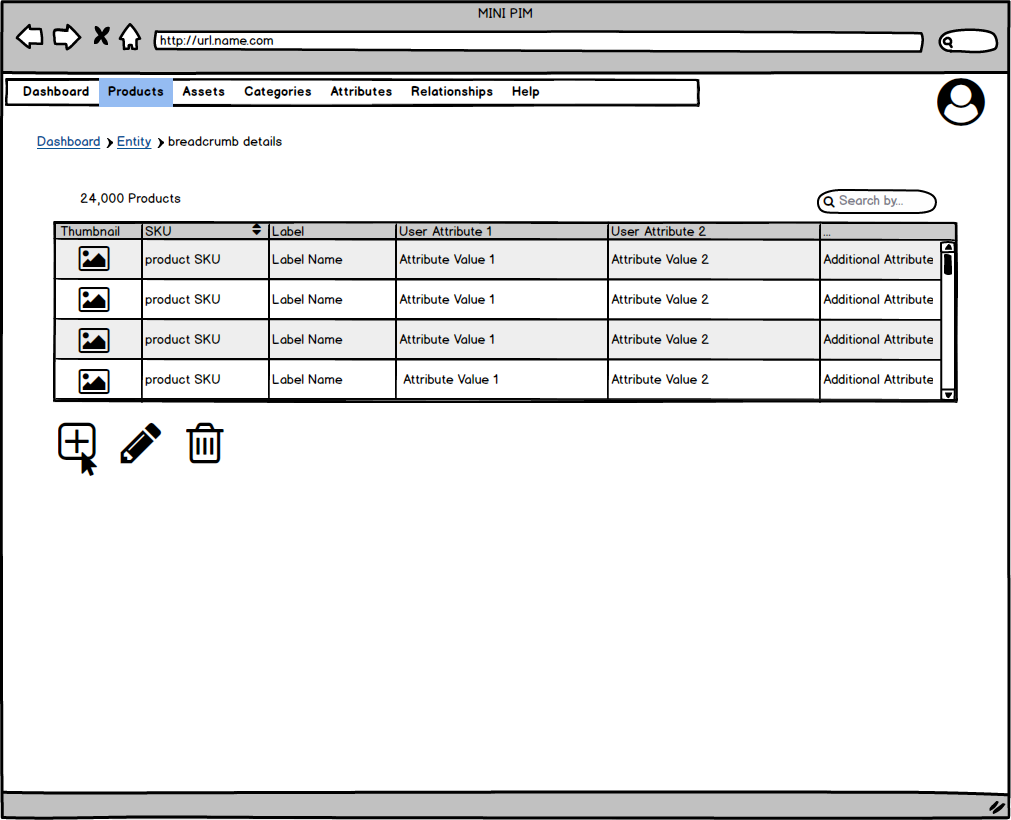
\includegraphics[width=1\linewidth]{mockups/RF2.1_boceto1.png}
    \caption{Apartado Productos hacer clic en \enquote{Añadir}}
   \end{figure}
\vspace{1.0cm}

\begin{figure}[H]
    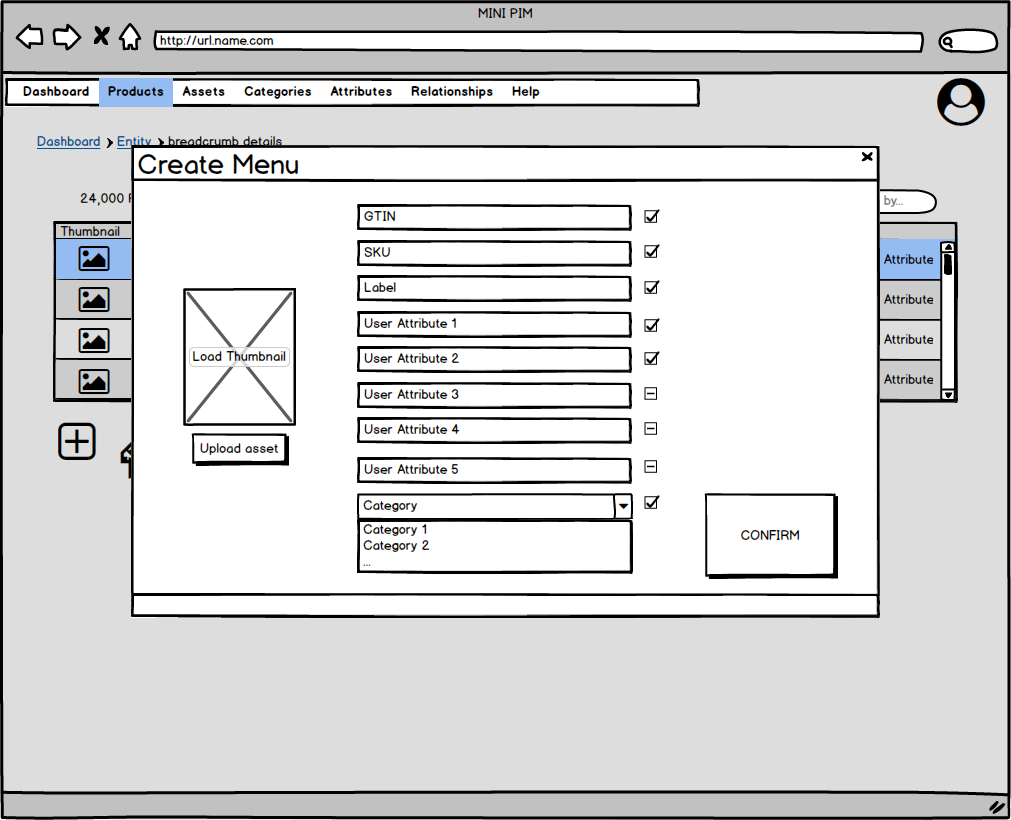
\includegraphics[width=1\linewidth]{mockups/RF2.1_bocetoCreacionV2.png}
    \caption{Menú de creación tras clicar \enquote{Añadir}}
   \end{figure}
\vspace{1.0cm}

\newpage %Inicia en una nueva página otro caso de uso
\phantomsection\numberedsection{RF2.1 Crear Producto}

\subsection*{Descripción}
Los usuarios deben de poder crear productos mientras sea posible, definiendo sus atributos y asignándoles sus respectivas categorías y relaciones.\par
\vspace{0.15cm}

\textbf{Pre-condición}\par
El usuario debe haber iniciado sesión en su cuenta en Mini PIM.\par
\vspace{0.15cm}

\textbf{Post-condición}
\begin{itemize}
    \item Caso de éxito: Todos los productos que el usuario creó se reflejan en la base de datos del sistema y en su interfaz gráfica.
    \item Caso mínimo: El sistema notifica al usuario el resultado de la acción de crear producto; exitosa o fallida.
\end{itemize}

\textbf{Prioridad: }
Alta
\vspace{0.15cm}

\textbf{Autor: }
Francisco Javier Jordá Garay\par
\vspace{0.15cm}

\textbf{Control de cambios: } Versión 1: Definición del caso de uso

\numberedsubsection{Escenario principal}
\begin{enumerate}
    \item El usuario se encuentra en el apartado de productos y selecciona la opción de \enquote{Añadir}.
    \item El sistema muestra el menú de creación solicitando al usuario:
    \begin{itemize}
        \item GTIN (atributo sistema $-$ comprueba validez de longitud)
        \item SKU (atributo sistema)
        \item Thumbnail (atributo sistema $-$ comprueba tamaño 200$\times$200px y formato)
        \item Label (atributo sistema $-$ comprueba máximo de 250 caracteres)
        \item Atributos (opcional $-$ comprueba máximo 5 nuevos atributos usuario)
        \item Categorías (opcional)
    \end{itemize}
    \item El usuario introduce los datos obligatorios y los que decida de opcionales y selecciona \enquote{Confirmar}.
    \item El sistema comprueba la validez de los datos introducidos por el usuario.
    \item El sistema almacena el producto creado en la base de datos registrando la fecha de creación.
    \item El sistema actualiza la información del total de datos registrados en la base de datos.
    \item El sistema muestra el apartado de \enquote{Productos} todos los recursos almacenados para esta sección.
\end{enumerate}

\numberedsubsection{Escenarios alternativos}
\begin{description}
    \item[2.a.] El sistema no puede almacenar el producto por superar el máximo de almacenamiento ligado al plan de suscripción del usuario.
    \begin{enumerate}
        \item[2.a.1] El sistema notifica al usuario que ha llegado al máximo de capacidad permitida en el plan de almacenamiento.
    \end{enumerate}

    \item[*.a] El usuario cancela la acción de crear un nuevo producto seleccionando la opción que cierra el menú de creación.
    \begin{enumerate}
        \item[*.a.1] El sistema regresa al apartado de \enquote{Productos}.
    \end{enumerate}

    \item[4.a] El sistema detecta un fallo en la comprobación de los datos obligatorios.
    \begin{enumerate}
        \item[4.a.1] El sistema notifica del error de comprobación al usuario mostrando el atributo del producto afectado.
        \item[4.a.2] El sistema regresa al menú de creación permitiendo edición de los datos.
    \end{enumerate}
\end{description}

\numberedsubsection{Casos de Prueba}
\underline{Escenario: Principal}\par
\vspace{0.15cm}
\textbf{Dado} que inicié sesión con mi cuenta de usuario correspondiente\par
\textbf{Y} estoy en el apartado de Productos\par
\textbf{Cuando} selecciono la opción de \enquote{Añadir}\par
\textbf{E} introduzco correctamente los atributos del producto que deseo crear\par
\textbf{Y} selecciono \enquote{confirmar} para guardar los datos\par
\textbf{Entonces} el sistema almacena la información en la base de datos de Mini PIM\par
\textbf{Y} actualiza la información del total de datos registrados en la base de datos\par
\textbf{Y} muestra el apartado de Productos con todos los recursos almacenados para esta sección.\par
\vspace{0.20cm}

\underline{Escenario: Alternativo 2.a}\par
\vspace{0.15cm}
\textbf{Dado} que inicié sesión con mi cuenta de usuario correspondiente\par
\textbf{Y} tengo el límite de productos\par
\textbf{Y} estoy en el apartado de Productos\par
\textbf{Cuando} selecciono la opción de \enquote{Añadir}\par
\textbf{E} introduzco correctamente los atributos del producto que deseo crear\par
\textbf{Y} selecciono \enquote{confirmar} para guardar los datos\par
\textbf{Entonces} el sistema me notifica que no puede almacenar el producto por superar el máximo de almacenamiento ligado a mi plan de suscripción actual\par
\vspace{0.20cm}

\underline{Escenario: Alternativo 3.a}\par
\vspace{0.15cm}
\textbf{Dado} que inicié sesión con mi cuenta de usuario correspondiente\par
\textbf{Y} estoy en el apartado de Productos\par
\textbf{Cuando} selecciono la opción de \enquote{Añadir}\par
\textbf{Y} selecciono la opción de cancelar\par
\textbf{Entonces} el sistema muestra el apartado de Productos mostrando todos los recursos almacenados sin ningún cambio.\par
\vspace{0.20cm}

\underline{Escenario: Alternativo 4.a}\par
\vspace{0.15cm}
\textbf{Dado} que inicié sesión con mi cuenta de usuario correspondiente\par
\textbf{Y} estoy en el apartado de Productos\par
\textbf{Cuando} selecciono la opción de \enquote{Añadir}\par
\textbf{Y} escribo los datos del producto y dejo uno obligatorio vacío\par
\textbf{Entonces} el sistema me muestra cual es el atributo que falla\par
\textbf{Y} regresa al menú de creación.\par
\vspace{0.20cm}

\numberedsubsection{Bocetos}
\begin{figure}[H]
    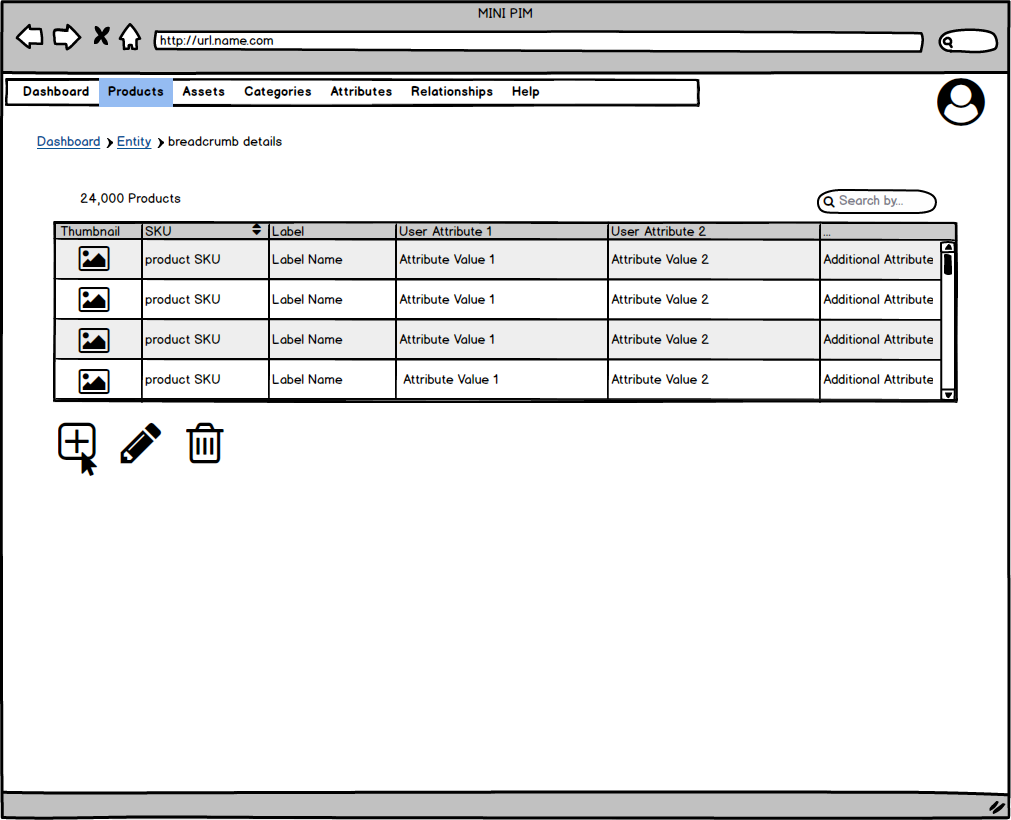
\includegraphics[width=1\linewidth]{mockups/RF2.1_boceto1.png}
    \caption{Apartado Productos hacer clic en \enquote{Añadir}}
   \end{figure}
\vspace{1.0cm}

\begin{figure}[H]
    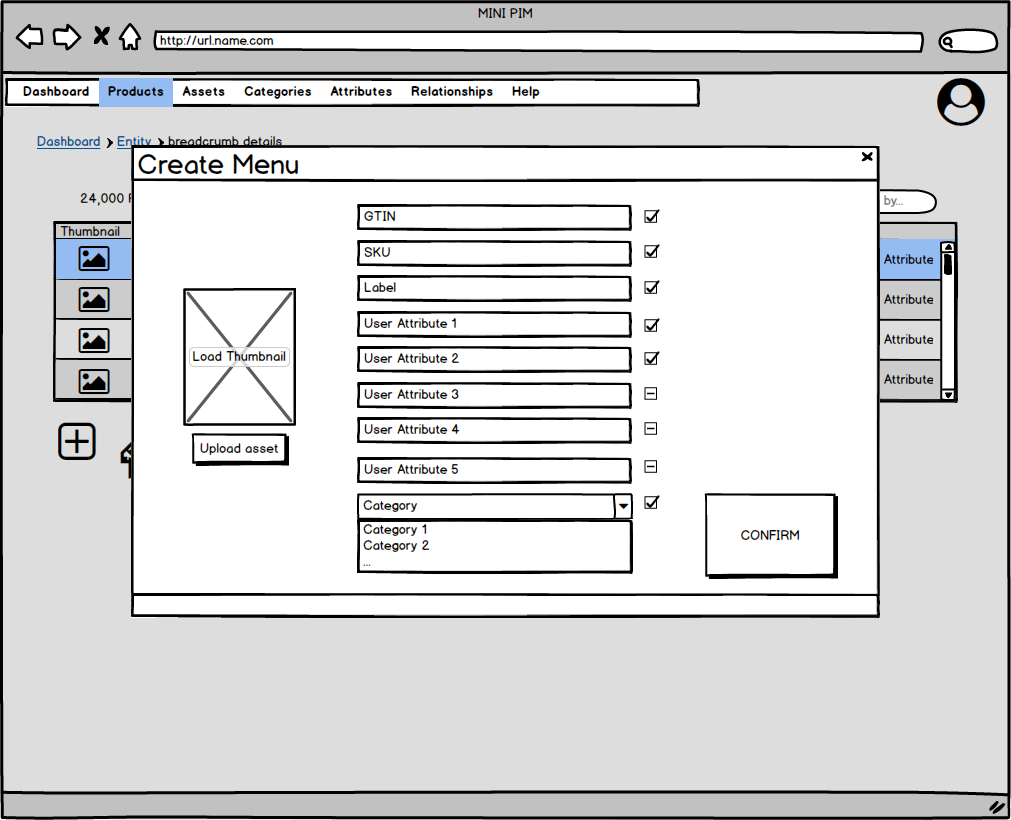
\includegraphics[width=1\linewidth]{mockups/RF2.1_bocetoCreacionV2.png}
    \caption{Menú de creación tras clicar \enquote{Añadir}}
   \end{figure}
\vspace{1.0cm}

\newpage %Inicia en una nueva página otro caso de uso
\phantomsection\numberedsection{RF2.1 Crear Producto}

\subsection*{Descripción}
Los usuarios deben de poder crear productos mientras sea posible, definiendo sus atributos y asignándoles sus respectivas categorías y relaciones.\par
\vspace{0.15cm}

\textbf{Pre-condición}\par
El usuario debe haber iniciado sesión en su cuenta en Mini PIM.\par
\vspace{0.15cm}

\textbf{Post-condición}
\begin{itemize}
    \item Caso de éxito: Todos los productos que el usuario creó se reflejan en la base de datos del sistema y en su interfaz gráfica.
    \item Caso mínimo: El sistema notifica al usuario el resultado de la acción de crear producto; exitosa o fallida.
\end{itemize}

\textbf{Prioridad: }
Alta
\vspace{0.15cm}

\textbf{Autor: }
Francisco Javier Jordá Garay\par
\vspace{0.15cm}

\textbf{Control de cambios: } Versión 1: Definición del caso de uso

\numberedsubsection{Escenario principal}
\begin{enumerate}
    \item El usuario se encuentra en el apartado de productos y selecciona la opción de \enquote{Añadir}.
    \item El sistema muestra el menú de creación solicitando al usuario:
    \begin{itemize}
        \item GTIN (atributo sistema $-$ comprueba validez de longitud)
        \item SKU (atributo sistema)
        \item Thumbnail (atributo sistema $-$ comprueba tamaño 200$\times$200px y formato)
        \item Label (atributo sistema $-$ comprueba máximo de 250 caracteres)
        \item Atributos (opcional $-$ comprueba máximo 5 nuevos atributos usuario)
        \item Categorías (opcional)
    \end{itemize}
    \item El usuario introduce los datos obligatorios y los que decida de opcionales y selecciona \enquote{Confirmar}.
    \item El sistema comprueba la validez de los datos introducidos por el usuario.
    \item El sistema almacena el producto creado en la base de datos registrando la fecha de creación.
    \item El sistema actualiza la información del total de datos registrados en la base de datos.
    \item El sistema muestra el apartado de \enquote{Productos} todos los recursos almacenados para esta sección.
\end{enumerate}

\numberedsubsection{Escenarios alternativos}
\begin{description}
    \item[2.a.] El sistema no puede almacenar el producto por superar el máximo de almacenamiento ligado al plan de suscripción del usuario.
    \begin{enumerate}
        \item[2.a.1] El sistema notifica al usuario que ha llegado al máximo de capacidad permitida en el plan de almacenamiento.
    \end{enumerate}

    \item[*.a] El usuario cancela la acción de crear un nuevo producto seleccionando la opción que cierra el menú de creación.
    \begin{enumerate}
        \item[*.a.1] El sistema regresa al apartado de \enquote{Productos}.
    \end{enumerate}

    \item[4.a] El sistema detecta un fallo en la comprobación de los datos obligatorios.
    \begin{enumerate}
        \item[4.a.1] El sistema notifica del error de comprobación al usuario mostrando el atributo del producto afectado.
        \item[4.a.2] El sistema regresa al menú de creación permitiendo edición de los datos.
    \end{enumerate}
\end{description}

\numberedsubsection{Casos de Prueba}
\underline{Escenario: Principal}\par
\vspace{0.15cm}
\textbf{Dado} que inicié sesión con mi cuenta de usuario correspondiente\par
\textbf{Y} estoy en el apartado de Productos\par
\textbf{Cuando} selecciono la opción de \enquote{Añadir}\par
\textbf{E} introduzco correctamente los atributos del producto que deseo crear\par
\textbf{Y} selecciono \enquote{confirmar} para guardar los datos\par
\textbf{Entonces} el sistema almacena la información en la base de datos de Mini PIM\par
\textbf{Y} actualiza la información del total de datos registrados en la base de datos\par
\textbf{Y} muestra el apartado de Productos con todos los recursos almacenados para esta sección.\par
\vspace{0.20cm}

\underline{Escenario: Alternativo 2.a}\par
\vspace{0.15cm}
\textbf{Dado} que inicié sesión con mi cuenta de usuario correspondiente\par
\textbf{Y} tengo el límite de productos\par
\textbf{Y} estoy en el apartado de Productos\par
\textbf{Cuando} selecciono la opción de \enquote{Añadir}\par
\textbf{E} introduzco correctamente los atributos del producto que deseo crear\par
\textbf{Y} selecciono \enquote{confirmar} para guardar los datos\par
\textbf{Entonces} el sistema me notifica que no puede almacenar el producto por superar el máximo de almacenamiento ligado a mi plan de suscripción actual\par
\vspace{0.20cm}

\underline{Escenario: Alternativo 3.a}\par
\vspace{0.15cm}
\textbf{Dado} que inicié sesión con mi cuenta de usuario correspondiente\par
\textbf{Y} estoy en el apartado de Productos\par
\textbf{Cuando} selecciono la opción de \enquote{Añadir}\par
\textbf{Y} selecciono la opción de cancelar\par
\textbf{Entonces} el sistema muestra el apartado de Productos mostrando todos los recursos almacenados sin ningún cambio.\par
\vspace{0.20cm}

\underline{Escenario: Alternativo 4.a}\par
\vspace{0.15cm}
\textbf{Dado} que inicié sesión con mi cuenta de usuario correspondiente\par
\textbf{Y} estoy en el apartado de Productos\par
\textbf{Cuando} selecciono la opción de \enquote{Añadir}\par
\textbf{Y} escribo los datos del producto y dejo uno obligatorio vacío\par
\textbf{Entonces} el sistema me muestra cual es el atributo que falla\par
\textbf{Y} regresa al menú de creación.\par
\vspace{0.20cm}

\numberedsubsection{Bocetos}
\begin{figure}[H]
    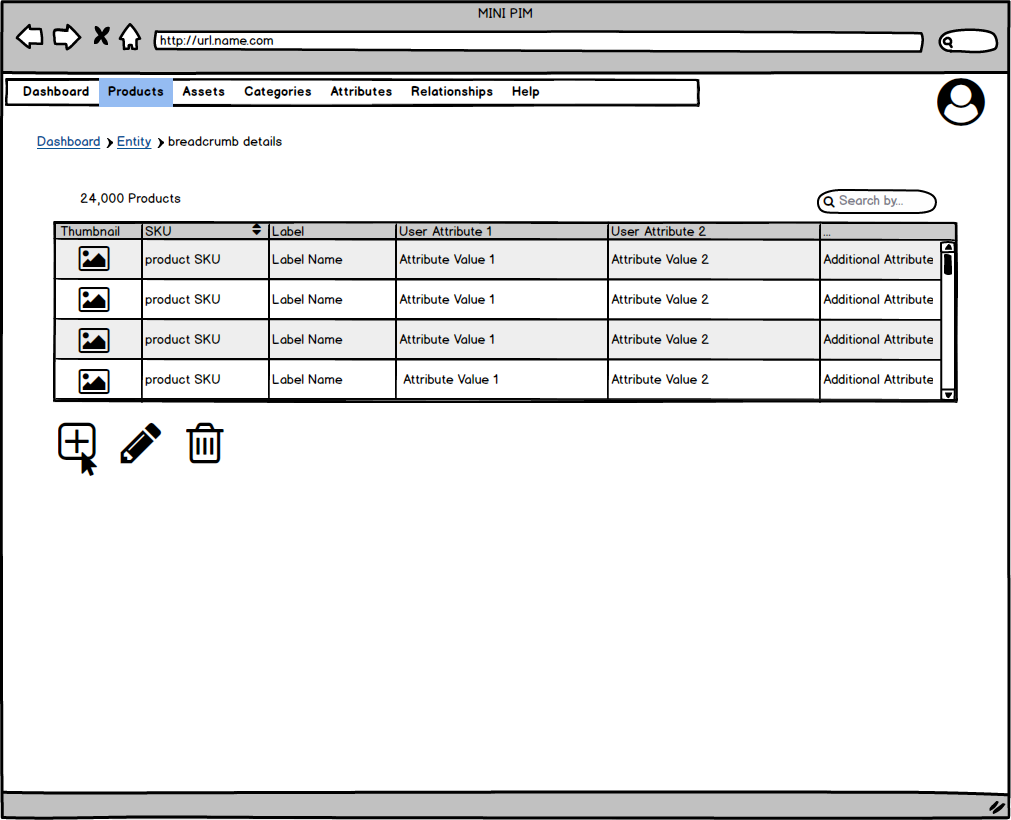
\includegraphics[width=1\linewidth]{mockups/RF2.1_boceto1.png}
    \caption{Apartado Productos hacer clic en \enquote{Añadir}}
   \end{figure}
\vspace{1.0cm}

\begin{figure}[H]
    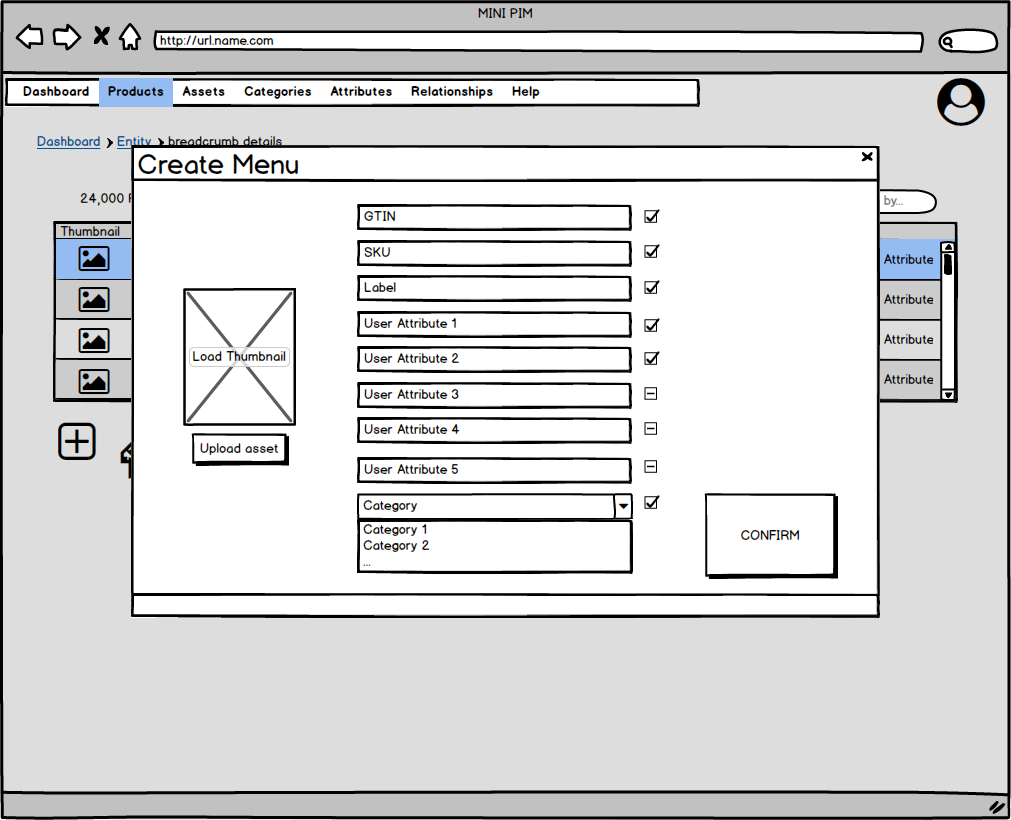
\includegraphics[width=1\linewidth]{mockups/RF2.1_bocetoCreacionV2.png}
    \caption{Menú de creación tras clicar \enquote{Añadir}}
   \end{figure}
\vspace{1.0cm}

\newpage %Inicia en una nueva página otro caso de uso
\phantomsection\numberedsection{RF2.1 Crear Producto}

\subsection*{Descripción}
Los usuarios deben de poder crear productos mientras sea posible, definiendo sus atributos y asignándoles sus respectivas categorías y relaciones.\par
\vspace{0.15cm}

\textbf{Pre-condición}\par
El usuario debe haber iniciado sesión en su cuenta en Mini PIM.\par
\vspace{0.15cm}

\textbf{Post-condición}
\begin{itemize}
    \item Caso de éxito: Todos los productos que el usuario creó se reflejan en la base de datos del sistema y en su interfaz gráfica.
    \item Caso mínimo: El sistema notifica al usuario el resultado de la acción de crear producto; exitosa o fallida.
\end{itemize}

\textbf{Prioridad: }
Alta
\vspace{0.15cm}

\textbf{Autor: }
Francisco Javier Jordá Garay\par
\vspace{0.15cm}

\textbf{Control de cambios: } Versión 1: Definición del caso de uso

\numberedsubsection{Escenario principal}
\begin{enumerate}
    \item El usuario se encuentra en el apartado de productos y selecciona la opción de \enquote{Añadir}.
    \item El sistema muestra el menú de creación solicitando al usuario:
    \begin{itemize}
        \item GTIN (atributo sistema $-$ comprueba validez de longitud)
        \item SKU (atributo sistema)
        \item Thumbnail (atributo sistema $-$ comprueba tamaño 200$\times$200px y formato)
        \item Label (atributo sistema $-$ comprueba máximo de 250 caracteres)
        \item Atributos (opcional $-$ comprueba máximo 5 nuevos atributos usuario)
        \item Categorías (opcional)
    \end{itemize}
    \item El usuario introduce los datos obligatorios y los que decida de opcionales y selecciona \enquote{Confirmar}.
    \item El sistema comprueba la validez de los datos introducidos por el usuario.
    \item El sistema almacena el producto creado en la base de datos registrando la fecha de creación.
    \item El sistema actualiza la información del total de datos registrados en la base de datos.
    \item El sistema muestra el apartado de \enquote{Productos} todos los recursos almacenados para esta sección.
\end{enumerate}

\numberedsubsection{Escenarios alternativos}
\begin{description}
    \item[2.a.] El sistema no puede almacenar el producto por superar el máximo de almacenamiento ligado al plan de suscripción del usuario.
    \begin{enumerate}
        \item[2.a.1] El sistema notifica al usuario que ha llegado al máximo de capacidad permitida en el plan de almacenamiento.
    \end{enumerate}

    \item[*.a] El usuario cancela la acción de crear un nuevo producto seleccionando la opción que cierra el menú de creación.
    \begin{enumerate}
        \item[*.a.1] El sistema regresa al apartado de \enquote{Productos}.
    \end{enumerate}

    \item[4.a] El sistema detecta un fallo en la comprobación de los datos obligatorios.
    \begin{enumerate}
        \item[4.a.1] El sistema notifica del error de comprobación al usuario mostrando el atributo del producto afectado.
        \item[4.a.2] El sistema regresa al menú de creación permitiendo edición de los datos.
    \end{enumerate}
\end{description}

\numberedsubsection{Casos de Prueba}
\underline{Escenario: Principal}\par
\vspace{0.15cm}
\textbf{Dado} que inicié sesión con mi cuenta de usuario correspondiente\par
\textbf{Y} estoy en el apartado de Productos\par
\textbf{Cuando} selecciono la opción de \enquote{Añadir}\par
\textbf{E} introduzco correctamente los atributos del producto que deseo crear\par
\textbf{Y} selecciono \enquote{confirmar} para guardar los datos\par
\textbf{Entonces} el sistema almacena la información en la base de datos de Mini PIM\par
\textbf{Y} actualiza la información del total de datos registrados en la base de datos\par
\textbf{Y} muestra el apartado de Productos con todos los recursos almacenados para esta sección.\par
\vspace{0.20cm}

\underline{Escenario: Alternativo 2.a}\par
\vspace{0.15cm}
\textbf{Dado} que inicié sesión con mi cuenta de usuario correspondiente\par
\textbf{Y} tengo el límite de productos\par
\textbf{Y} estoy en el apartado de Productos\par
\textbf{Cuando} selecciono la opción de \enquote{Añadir}\par
\textbf{E} introduzco correctamente los atributos del producto que deseo crear\par
\textbf{Y} selecciono \enquote{confirmar} para guardar los datos\par
\textbf{Entonces} el sistema me notifica que no puede almacenar el producto por superar el máximo de almacenamiento ligado a mi plan de suscripción actual\par
\vspace{0.20cm}

\underline{Escenario: Alternativo 3.a}\par
\vspace{0.15cm}
\textbf{Dado} que inicié sesión con mi cuenta de usuario correspondiente\par
\textbf{Y} estoy en el apartado de Productos\par
\textbf{Cuando} selecciono la opción de \enquote{Añadir}\par
\textbf{Y} selecciono la opción de cancelar\par
\textbf{Entonces} el sistema muestra el apartado de Productos mostrando todos los recursos almacenados sin ningún cambio.\par
\vspace{0.20cm}

\underline{Escenario: Alternativo 4.a}\par
\vspace{0.15cm}
\textbf{Dado} que inicié sesión con mi cuenta de usuario correspondiente\par
\textbf{Y} estoy en el apartado de Productos\par
\textbf{Cuando} selecciono la opción de \enquote{Añadir}\par
\textbf{Y} escribo los datos del producto y dejo uno obligatorio vacío\par
\textbf{Entonces} el sistema me muestra cual es el atributo que falla\par
\textbf{Y} regresa al menú de creación.\par
\vspace{0.20cm}

\numberedsubsection{Bocetos}
\begin{figure}[H]
    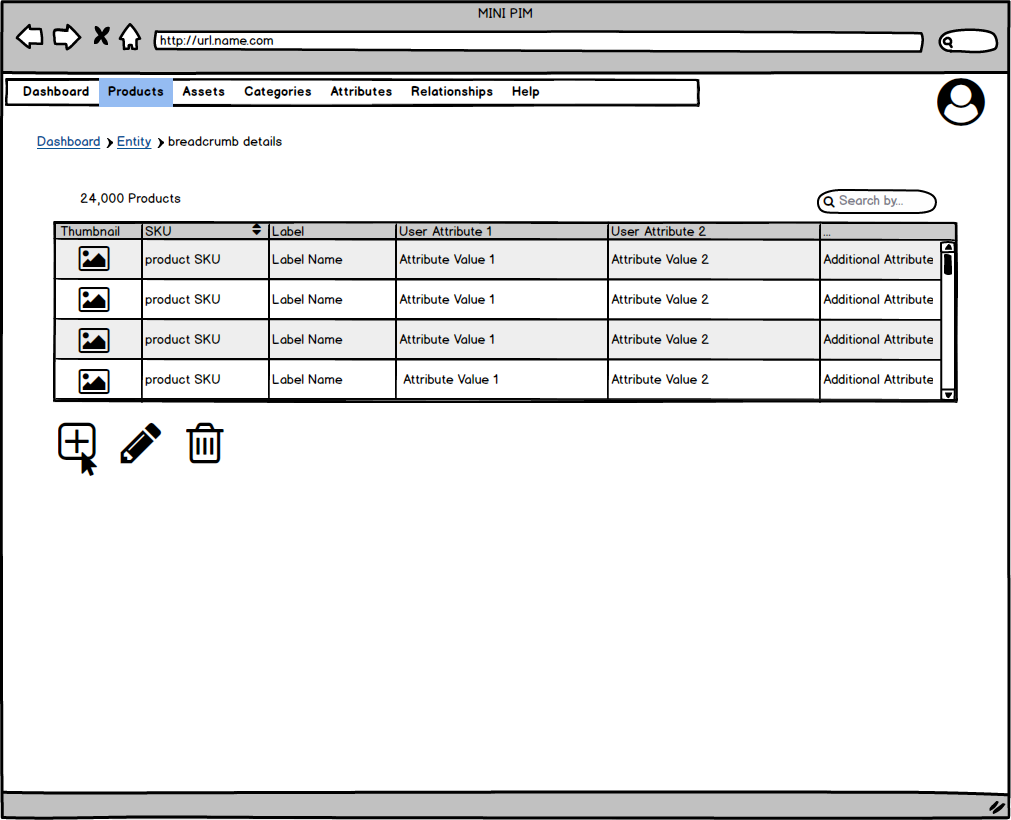
\includegraphics[width=1\linewidth]{mockups/RF2.1_boceto1.png}
    \caption{Apartado Productos hacer clic en \enquote{Añadir}}
   \end{figure}
\vspace{1.0cm}

\begin{figure}[H]
    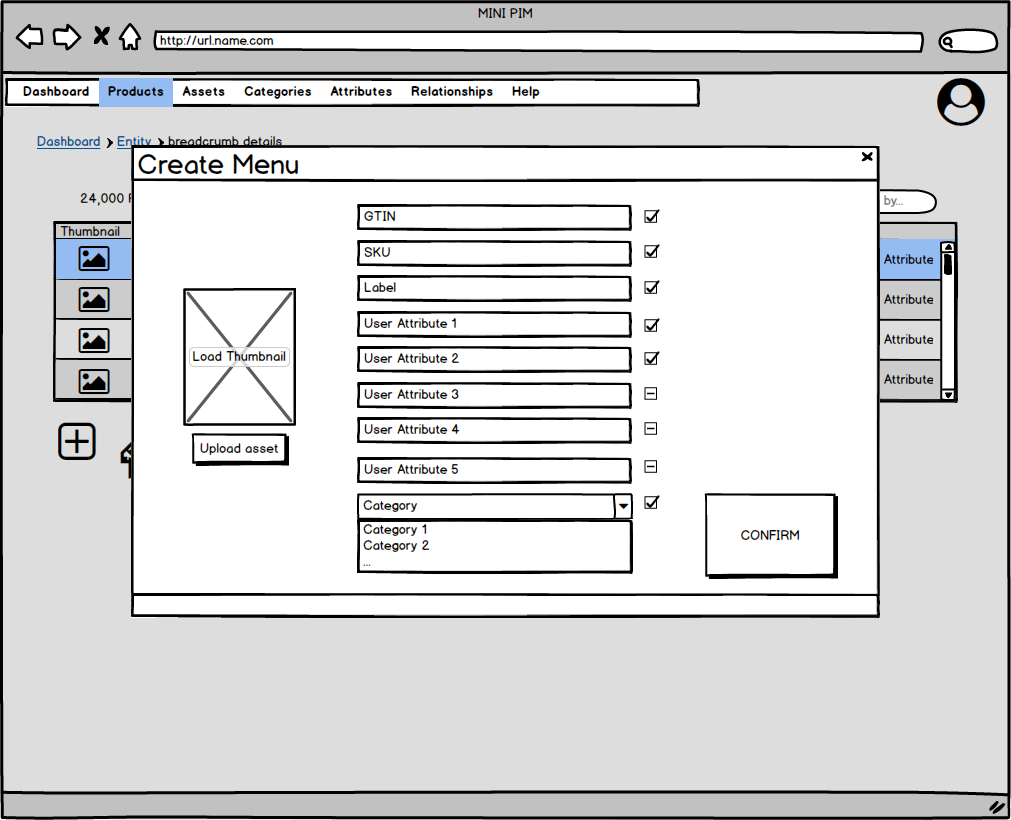
\includegraphics[width=1\linewidth]{mockups/RF2.1_bocetoCreacionV2.png}
    \caption{Menú de creación tras clicar \enquote{Añadir}}
   \end{figure}
\vspace{1.0cm}

\newpage %Inicia en una nueva página otro caso de uso



\end{document}